\documentclass{tufte-handout}

%\geometry{showframe}% for debugging purposes -- displays the margins



\newcommand{\bra}[1]{\left(#1\right)}
\usepackage{clrscode3e}
\usepackage[activate={true,nocompatibility},final,tracking=true,kerning=true,spacing=true,factor=1100,stretch=10,shrink=10]{microtype}
\usepackage{tikz}
\usepackage{amsmath,amsthm}
\usetikzlibrary{shapes}
\usetikzlibrary{positioning}
% Set up the images/graphics package
\usepackage{graphicx}
\setkeys{Gin}{width=\linewidth,totalheight=\textheight,keepaspectratio}
\graphicspath{{.}}

\title{Lecture Notes for MATH 350 - Fall 2017}
\author[Ralph Sarkis]{Ralph Sarkis}
\date{\today}  % if the \date{} command is left out, the current date will be used

% The following package makes prettier tables.  We're all about the bling!
\usepackage{booktabs}

% The units package provides nice, non-stacked fractions and better spacing
% for units.
\usepackage{units}

% The fancyvrb package lets us customize the formatting of verbatim
% environments.  We use a slightly smaller font.
\usepackage{fancyvrb}
\fvset{fontsize=\normalsize}

% Small sections of multiple columns
\usepackage{multicol}

%--------Theorem Environments--------
%theoremstyle{plain} --- default
\newtheorem{thm}{Theorem}
\newtheorem{cor}[thm]{Corollary}
\newtheorem{prop}[thm]{Proposition}
\newtheorem{lem}[thm]{Lemma}
\newtheorem{conj}[thm]{Conjecture}
\newtheorem{quest}[thm]{Question}
\newtheorem{claim}{Claim}

\theoremstyle{definition}
\newtheorem{defn}[thm]{Definition}
\newtheorem{defns}[thm]{Definitions}
\newtheorem{con}[thm]{Construction}
\newtheorem{exmp}[thm]{Example}
\newtheorem{jk}[thm]{Joke}
\newtheorem{exmps}[thm]{Examples}
\newtheorem{notn}[thm]{Notation}
\newtheorem{notns}[thm]{Notations}
\newtheorem{addm}[thm]{Addendum}
\newtheorem{exer}[thm]{Exercise}

\theoremstyle{remark}
\newtheorem{rem}[thm]{Remark}
\newtheorem{ans}[thm]{Answer}
\newtheorem{rems}[thm]{Remarks}
\newtheorem{warn}[thm]{Warning}
\newtheorem{sch}[thm]{Scholium}

\newcommand{\Mod}[1]{\ (\text{mod}\ #1)}
\newcommand{\R}{\mathbb{R}}
\newcommand{\N}{\mathbb{N}}
\newcommand{\Q}{\mathbb{Q}}
\newcommand{\F}{\mathbb{F}}
\newcommand{\Z}{\mathbb{Z}}
\renewcommand{\P}{\mathbb{P}}
\DeclareMathOperator{\Span}{Span}
\DeclareMathOperator{\val}{val}
\DeclareMathOperator{\comp}{comp}
\DeclareMathOperator{\im}{Im}
\DeclareMathOperator{\reg}{Reg}
\DeclareMathOperator{\odd}{Odd}
\DeclareMathOperator{\dist}{dist}
\DeclareMathOperator{\sbd}{sbd}
\DeclareMathOperator{\capac}{cap}


% These commands are used to pretty-print LaTeX commands
\newcommand{\doccmd}[1]{\texttt{\textbackslash#1}}% command name -- adds backslash automatically
\newcommand{\docopt}[1]{\ensuremath{\langle}\textrm{\textit{#1}}\ensuremath{\rangle}}% optional command argument
\newcommand{\docarg}[1]{\textrm{\textit{#1}}}% (required) command argument
\newenvironment{docspec}{\begin{quote}\noindent}{\end{quote}}% command specification environment
\newcommand{\docenv}[1]{\textsf{#1}}% environment name
\newcommand{\docpkg}[1]{\texttt{#1}}% package name
\newcommand{\doccls}[1]{\texttt{#1}}% document class name
\newcommand{\docclsopt}[1]{\texttt{#1}}% document class option name

\begin{document}

\maketitle
\begin{abstract}
These are my lecture notes taken during the Introduction to graph theory class in fall 2017.
\end{abstract}
\tableofcontents
\section{Course Introduction}
This class will be taught by Jan Volec. There will be 10 assignments with one warm-up question and a challenge question on each which will not be graded. Both the midterm and the final will be open-book exams. The weights of the assignments will be 20\%, the weights of the midterm will be 20\% and the weight of the final will be 60\%. The office hours of Jan Volec are on Tuesday from 10:30 to 12:30 in Burnside 1242. There is more information on Jan Volec's website at \verb|http://honza.ucw.cz|.

\section{Introduction to graphs}
\begin{defn}[Graph]
	A \textbf{graph} $G$ is an ordered pair with a set of vertices $V$ and a set of edges $E \subseteq \binom{V}{2}$\footnote{Here the binomial notation $\binom{S}{k}$ where $S$ is a set and $k \in \N$ denotes the set of unordered $k-tuples$ with elements in $S$}. $V$ is normally finite and $E$ is a set of unordered pair of vertices. $E$ can sometimes be considered as a multi-set so that you can have multiple edges which are the same.
\end{defn}
\begin{marginfigure}
	\centering
	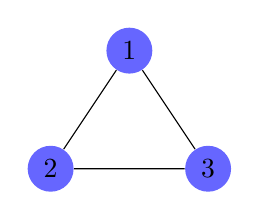
\begin{tikzpicture}[main_node/.style={circle,fill=blue!60,minimum size=1em,inner sep=3pt}]
		
		\node[main_node] (1) at (0,0) {$1$};
		\node[main_node] (2) at (-1, -1.5)  {$2$};
		\node[main_node] (3) at (1, -1.5) {$3$};
		
		\draw (1) -- (2) -- (3) -- (1);
	\end{tikzpicture}
\caption{This represents the graph $G = \bra{V,E}$ where $V = \{1,2,3\}$ and $E = \left\lbrace \{1,2\}, \{2,3\}, \{3,1\} \right\rbrace$}
\label{fig:exgraph}
\end{marginfigure}
\begin{exmp}
	See figure \ref{fig:exgraph}.
\end{exmp}

Before actually diving into the formal theory of graphs, we look at simple problems that were solved using graph theory (simple in their formulation, not necessarily their solution).

\begin{enumerate}
	\item How can you connect houses on an electrical grid with the least amount of wires ?
	
	The first algorithm to solve this problem was designed by Otakar Bor\r{u}vka in 1926.
	
	\item What is the shortest distance you can travel while visiting all 647 U.S. colleges exactly once ?
	
	The tour was found in 2015 by William Cook from UW.
	
	\begin{marginfigure}
		\centering
		\includegraphics{Konigsberg_bridges}
		\caption{The seven bridges of K\"onigsberg puzzle}
		\label{fig:konig}
	\end{marginfigure}
	\item Can you cross the seven bridges of K\"onigsberg exactly once ? (See figure \ref{fig:konig}.)
	
	The answer is no and it was proved by Euler. Draw each part of land separated by the river as a node of a graph, and draw the bridges as edges between the nodes. Observe that more than 2 nodes have an odd amount of edges. However, all nodes which are not the start or end of the tour must have an even amount of edges, because if you come on the land from a bridge, you must leave from another bridge. Hence, we can have at most 2 nodes with uneven edges connected, which is not the case in K\"onigsberg puzzle.
	
	\item How can you disconnect 2 railway networks by destroying the least amount of connections between towns ?
	
	There are secret reports from 1955 that show the solution to this problem on the railway network connecting the Soviet Union to East Europe.
	
	\item Let there be a town with several factories and stores with roads connecting them. There are 3 rules for the roads.
	\begin{itemize}
		\item No road can connect 2 stores.
		\item No road can connect 2 factory.
		\item There can be intersection between roads.
	\end{itemize}
	Can there be simultaneously more than 2 factories and more than 2 stores ?
	
	No, it is not possible.
	
	\item You have eight batteries in your bag and you know that four of them work (you do not know which work or which do not work). You need two charged batteries to power a GPS. What is the best strategy to switch batteries in the device the least amount of time before being sure to have two charged batteries ?
	
	Make a two groups of three batteries and try every possible combination in each groups (maximum six trials). If no combination worked, the two batteries outside of the group are charged and so you have a total of seven trials. The general solution for this problem is known if you need two batteries but not if you need three.
	
	\item Is every political map 4-colorable ? You color a map with four colors and each country is colored so that no adjacent countries have the same colors.
	
	This is the first accepted proof that was computer assisted. It is really big and considers lots of cases (that is why a computer was needed). Note that the proof for 6-colorable is almost trivial.
	
	\item In a graph with 20 vertices, you can always find 4 vertices which are either not connected or all connected.
	
	This is part of Ramsey theory which gives motivation for the Ramsey numbers. The following remark is a result easier to prove than the one above.
	
	\begin{rem}
		In a complete graph with 6 vertices and 2 colors of edges (red and blue), you can always find a red triangle or a blue triangle.
	\end{rem}
	\begin{proof}
		Take an arbitrary node in the graph, call it $A$. Assume $A$ has at least three blue edges, then between nodes connected connected to $A$ via blue edges there are two possibilities. If there is a blue connection between these nodes, we obtain a blue triangle with $A$, if there is no blue connection, we obtain a red triangle. If $A$ has less than three blue edges, then it has at least three red edges and the same argument as above holds.
	\end{proof}
\end{enumerate}

We will now give several vocabulary definitions that we will often use in the course.

\begin{defns}[Vocabulary of graphs]
	Let $G = (V,E)$ be a graph.
	\begin{itemize}
		\item Let $e_1,e_2 \in E$ be two edges, we say that they are \textbf{parallel} if they join the same pair of vertices.
		\item Let $e \in E$ be an edge, we say that it is a \textbf{loop} if it connects a vertex to itself.
		\item Let $e = \{u,v\} \in E$ where $u,v \in V$, we say that $u$ and $v$ are the \textbf{endpoints} or \textbf{ends} of $e$.
		\item $G$ is called \textbf{simple} if it contains no parallel edges and no loops. It is called loopless if it has no loops.
		\item \textbf{Non-simple} graphs are also called \textbf{multi-graph}.
		\item We use the following notation when working with multiple graphs : $V(G) = V$ and $E(G) = E$.
		\item Let $u,v \in V$, we say that $u$ and $v$ are \textbf{adjacent} if there exists an edge $e \in E$ of which they are the endpoints.
		\item Let $v \in V$ and $e \in E$, we say that $e$ is \textbf{incident} to $v$ or that $v$ is \textbf{incident} to $e$ if $v$ is an endpoint of $e$.
		\item Let $e_1, e_2 \in E$ be two edges, we say that they are \textbf{coincident} if the share a common endpoint.
		\item The \textbf{degree} of a vertex $v \in V$ is defined by the number of edges incident to $v$. It is denoted $\deg{\bra{v}}$.
	\end{itemize}
\end{defns}

We will take a small break from these definitions to prove a simple lemma and its corollary.

\begin{lem}[Handshaking lemma]
	For every graph $G = (V,E)$, the sum of the degrees of all the vertices is even.
\end{lem}
\begin{cor}
	The number of vertices with odd degrees is even.
\end{cor}
\begin{proof}[Proof of corollary]
	Let $V_0 =\{v \in V \mid \deg{\bra{v}} \equiv 0 \Mod{2}\}$ and $V_1 = \{v \in V \mid \deg{\bra{v}} \equiv 1 \Mod{2}\}$, we decompose the summation of all degrees like so:
	\[ \sum_{v \in V} \deg{\bra{v}} = \sum_{v \in V_0} \deg{\bra{v}} + \sum_{v \in V_1} \deg{\bra{v}} \]
	The summation in $V_0$ is even and since the left hand side is even, the summation in $V_1$ must be even. Hence, $\left|V_1\right|$ must be even. 
\end{proof}
\marginnote{The proof technique we are using here, namely counting the same thing in 2 different ways, is often used in proofs about graphs}
\begin{proof}[Proof of lemma]
	By the definition of degree, we can infer that each time a vertex $v$ is an endpoint of an edge, its degree is incremented (loop edges count twice for the same vertex). Thus, the summation is equal to the number of endpoints or twice the number of edges (an even number).
\end{proof}

Back to definitions now. When working with simple graphs, we can define really useful matrices.

\begin{defn}[Adjacency matrix]
	Let $G = (V,E)$ be a graph with $V = \{v_1, \cdots, v_n\}$, the \textbf{adjacency matrix} is defined by $A = \bra{a_{ij}}$ where $a_{ij} = \begin{cases}1 & \{v_i, v_j\} \in E\\ 0 & \mbox{ otherwise}\end{cases}$
\end{defn}
\begin{marginfigure}
	\centering
	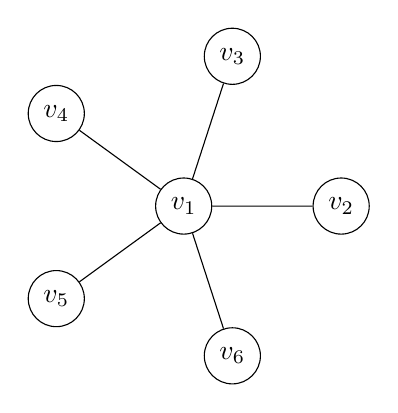
\begin{tikzpicture}[scale=2]
	\tikzstyle{every node}=[draw,shape=circle];
	\path (0:0cm)    node (v0) {$v_1$};
	\path (0:1cm)    node (v1) {$v_2$};
	\path (72:1cm)   node (v2) {$v_3$};
	\path (2*72:1cm) node (v3) {$v_4$};
	\path (3*72:1cm) node (v4) {$v_5$};
	\path (4*72:1cm) node (v5) {$v_6$};
	\draw (v0) -- (v1)
	(v0) -- (v2)
	(v0) -- (v3)
	(v0) -- (v4)
	(v0) -- (v5);
	\end{tikzpicture}
	\caption{Example of a simple graph}
	\label{fig:star}
\end{marginfigure}

\begin{exmp}
	For the graph in figure \ref{fig:star}, the adjacency matrix is the following:
	\[
		\begin{bmatrix}
			0 & 1 & 1 & 1 & 1 & 1\\
			1 & 0 & 0 & 0 & 0 & 0\\
			1 & 0 & 0 & 0 & 0 & 0\\
			1 & 0 & 0 & 0 & 0 & 0\\
			1 & 0 & 0 & 0 & 0 & 0\\
			1 & 0 & 0 & 0 & 0 & 0\\
		\end{bmatrix}
	\]
\end{exmp}
\marginnote{Note that the adjacency matrix is always a $n\times n$ symmetric because when $v_i$ is adjacent to $v_j$, the other way is true as well}
\begin{defn}[Incidence matrix]
	Let $G = (V, E)$ be a graph with $V = \{v_1, \dots, v_n\}$, the \textbf{incidence matrix} is defined by $B = \bra{b_{ij}}$ where $b_{ij} = \begin{cases}1 & e_j \mbox{ is incident to } v_i\\ 0 & \mbox{ otherwise}\end{cases}$
\end{defn}
\begin{exmp}
	For the graph in Figure 3., we denote $e_1$ to be the edge going from $v_1$ to $v_2$ and increment the subscript counter clockwise, the incidence matrix is the following:
	\[
		\begin{bmatrix}
			1 & 1 & 1 & 1 & 1\\
			1 & 0 & 0 & 0 & 0\\
			0 & 1 & 0 & 0 & 0\\
			0 & 0 & 1 & 0 & 0\\
			0 & 0 & 0 & 1 & 0\\
			0 & 0 & 0 & 0 & 1\\
		\end{bmatrix}
	\]
\end{exmp}
The intuition for the adjacency matrix is that is shows which edges are connected to together\footnote{I did not find a nice intuition for the incidence matrix, maybe we will see more of it in the class}. Since, we are familiar with matrices from linear algebra, there are natural questions we can ask.

\begin{quest}
	What does $A \cdot A$ mean ? (where $A$ is the adjacency matrix and $\cdot$ is the usual matrix product)
\end{quest}
\begin{ans}
	Obviously, it is a $n\times n$ matrix and we have $A^2 = \bra{a_{ij}}$, where $a_{ij}$ is the number of walks from $v_i$ to $v_j$ with distance 2. A consequence of that is that the diagonal is the degrees of the vertices, namely, $a_{ii} = \deg{\bra{v_i}}$.
\end{ans}
\begin{quest}
	What does $B \cdot B^{T}$ mean ? (where $B$ is the incidence matrix)
\end{quest}
\begin{ans}
	We end up with a $n\times n$ matrix and we have $$B\cdot B^{T} = A + \text{diag}\bra{\deg{\bra{v_1}}, \dots, \deg{\bra{v_n}}}$$
\end{ans}

We talked about a walk in the first answer and you can actually have an intuition about what a walk is on a graph but we will define it in a formal way along with other similar definitions.

\begin{defn}[Walk]
	Let $G = (V, E)$ be a graph, a \textbf{walk} on $G$ is a sequence $\{v_0, e_1, v_1, \dots, e_k, v_k\}$ where $\forall i \in \N, v_i \in V, e_i \in E$ with the property that $\forall i \geq 1, e_i = \{v_{i-1}, v_i\}$.
\end{defn}
\begin{defn}
	$\sim_G^W$\footnote{We use the $W$ superscript to specify that is a walking relation} is a relation on $V(G)$ with $u \sim_G^W v$ if and only if there exists a walk on $G$ from $u$ to $v$.
\end{defn}
\begin{defn}[Trail]
	Let $G = (V, E)$ be a graph, a \textbf{trail} on $G$ is a walk on $G$ with the property that no edge is repeated.
\end{defn}
\begin{defn}
	$\sim_G^T$ is a relation on $V(G)$ with $u \sim_G^W v$ if and only if there exists a trail from $u$ to $v$.
\end{defn}
\begin{defn}[Path]
Let $G = (V, E)$ be a graph, a \textbf{path} on $G$ is a walk on $G$ with the property that no vertex is repeated\footnote{A consequence is that no edge is repeated so every path is a trail}.
\end{defn}
\begin{defn}
$\sim_G^T$ is a relation on $V(G)$ with $u \sim_G^W v$ if and only if there exists a trail from $u$ to $v$.
\end{defn}

The next proposition will show that these three relations are redundant and that we will only need one of them.
\begin{prop}
	All these relations are the same, namely, the existence of walk guarantees the existence of a trail which guarantees the existence of a path which guarantees the existence of a walk.
\end{prop}
Before proving it, we prove a corollary which motivates the definition of these relations.
\begin{cor}
	For any graph $G$, the walk, trail and path relations are equivalence relations on $V(G)$.
\end{cor}
\begin{proof}
	Let $G = (V,E)$ be a graph and $u,v,w \in V$ be vertices. Using the proposition, we only need to prove it for a walk. The walk relation is symmetric because if there exists a walk from $u$ to $v$, the reversed sequence is a walk from $v$ to $u$. It is also reflexive because ${u}$ is always a valid walk from $u$ to $u$. To prove transitivity, assume that $u \sim_G^W v$ and $v \sim_G^W w$, then there exists sequences $\{u, e_1, v_1, \dots, e_m, v\}$ and $\{v, e'_1, v'_1, \dots, e'_n, w\}$ that represent walks on $G$. Indeed, we can create a new walk $\{u, e_1, v_1, \dots, e_m, v, e'_1, v'_1, \dots, e'_n, w\}$ from $u$ to $w$.
\end{proof}
\begin{proof}[Proof of the proposition]
	We will show that if a walk exists between $u,v \in V(G)$ for an arbitrary graph $G$, a path also exists from $u$ to $v$. The other directions we need for equivalence between walk, trail and path are all trivial. Suppose that there exists a walk from $u$ to $v$, then we can find the smallest walk $W = \{w_0, e_1, w_1, e_2, \dots, e_n, w_n\}$ where $w_0 = u$ and $w_n = v$\footnote{A formal argument for that would be to use the well-ordering principle on the set of sizes of walks from $u$ to $v$}. We claim that this walk is a path. Assume that for some $1 \leq i < j \leq n$, $w_i = w_j$. Then, we can construct a smaller walk $W' = \{w_0, e_1, w_1, \dots, e_i, w_i, e_{j+1}, w_{j+1}, \dots, w_n\}$ that still goes from $u$ to $v$, contradicting our choice of $W$. Since, $W$ does not have a repeated vertex, it is a path.
\end{proof}

\begin{defn}[Connected components]
	The equivalence classes defined by the $\sim_G$ relation are called \textbf{connected components}. See figure \ref{fig:comps} for an example. For some graph $G$, the number of connected components in the graph is denoted $\comp(G)$. We say that a graph $G$ is \textbf{connected} if $\comp(G) = 1$.
\end{defn}
\begin{marginfigure}
	\centering
	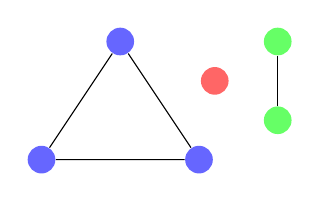
\begin{tikzpicture}[scale=1,bnode/.style={circle,fill=blue!60,minimum size=1em,inner sep=1pt}, rnode/.style={circle,fill=red!60,minimum size=1em,inner sep=1pt}, gnode/.style={circle,fill=green!60,minimum size=1em,inner sep=1pt}]
	
	\node[bnode] (1) at (0,0) {};
	\node[bnode] (2) at (-1, -1.5)  {};
	\node[bnode] (3) at (1, -1.5) {};
	
	\node[gnode] (4) at (2,0) {};
	\node[gnode] (5) at (2, -1)  {};
	
	\node[rnode] (6) at (1.2, -0.5) {};
	
	\draw (1) -- (2) -- (3) -- (1);
	\draw (4) -- (5);
	\end{tikzpicture}
	\caption{The connected components of this graph each have different colors}
	\label{fig:comps}
\end{marginfigure}
To formalize some of the concepts we described above, we sometimes use the notion of subgraphs.
\begin{defn}[Subgraph]
	Let $G = (V,E)$ be a graph. We say that a graph $H = (V', E')$ is a \textbf{subgraph} of $G$ if $V' \subseteq V$ and $E' \subseteq E \cap \binom{V'}{2}$. In other words, all the vertices in $H$ must be in $G$ and all the edges in $H$ must be in $G$ and incident to the vertices in $H$. We say that a subgraph $H$ of $G$ is induced if $E(H) = E(G) \cap \binom{V(H)}{2}$.
\end{defn}
\begin{rem}
	For a graph $G = (V,E)$, a vertex-maximal subgraph of $G$ that is connected is a connected subgraph for which you cannot add a node from $G$ and still get a connected subgraph. Notice that any vertex-maximal subgraph of $G$ is a connected component of $G$.
\end{rem}

Here we present some common examples of graphs.
\begin{exmps}
	\begin{enumerate}
		\item[]
		\item The null graph is a graph with no vertices and no edges : $G = (\emptyset, \emptyset)$.
		\item The empty graph on $n$ vertices is $E_n = (V, \emptyset)$ where $V = \{1,\dots, n\}$.
		\item The complete graph on $n$ vertices is $\overline{E_n} = K_n = (V, E)$ where $V = \{1,\dots, n\}$ and $E = \binom{V}{2}$.
		\item A path on $n$ vertices is $P_n = (V,E)$ where $V = \{1,\dots, n\}$ and $E = \{e_1, \dots, e_{n-1}\}$ with $e_i = \{i, i+1\}$ for $i \in \{1,\cdot, n-1\}$.
		\item A cycle on $n$ vertices is $C_n = (V,E)$ where $V = \{1,\dots, n\}$ and $E = \{e_1, \dots, e_{n}\}$ with $e_i = \{i, i+1\}$ for $i \in \{1,\cdot, n-1\}$ and $e_n = \{n, 1\}$.
	\end{enumerate}
\end{exmps}
\begin{rem}
	When we talk about the length of paths or cycles, we will refer to the number of edges in the path/cycle.
\end{rem}

When working with graphs, we sometimes need to compare them and say that they are "equal". We formalize this with the notion of isomorphism.

\begin{defn}[Graph isomorphism]
	Let $G$ and $H$ be graphs, we say that $G$ is \textbf{isomorphic} to $H$\footnote{We often make an abuse of vocabulary and just say that $G$ is $H$} and denote it $G \simeq H$ if there exists a bijection $f: V(G) \rightarrow V(H)$ such that $\{u,v\} \in E(G) \Leftrightarrow \{f(u), f(v)\} \in E(H)$. In simpler terms, we just want to be able to rearrange the representation of $G$ so that it looks like the representation of $H$.
\end{defn}
\begin{rem}
	In this course, when we talk about any graph, we are in fact talking about all the graphs that are isomorphic to it (i.e: we never make distinctions between graphs that are isomorphic).
\end{rem}

We quickly go back to the notion of connected components and prove an interesting result.

\begin{defn}
	Let $G = (V,E)$ be a graph. For some $e \in E$, we denote $G-e$ to be the graph $G$ with the edge $e$ removed. Namely, $G-e = (V,E')$ with $E' = E \setminus \{e\}$.
\end{defn}
\begin{defn}[Cut edge]
	An edge $e \in E(G)$ is a \textbf{cut edge} if $$\comp{(G-e)} = \comp{(G)} + 1$$.
\end{defn}
\begin{lem}
	Let $G$ be a graph, $e \in E(G)$ is a cut edge if and only if there is no cycle in $G$ containing $e$.
\end{lem}
\begin{proof}
	($\Rightarrow$) Denote $e = \{u,v\}$, we know that $G-e$ has one more connected component than $G$. This implies that in $G-e$, the vertex $u$ is in a different component than $v$. Assume towards a contradiction that there is a cycle containing $e$, we can write it as $C = \{v_1, e_1, v_2, \dots, v_k, e_k, v_1\}$ where $v_1 = u$, $v_k = v$ and $e_k = e$. Now, we can construct a path $P = \{v_1, e_1, \cdots, v_k\}$ which is valid in $G-e$ but this contradicts the fact that $u$ and $v$ are not connected.
	
	($\Leftarrow$) If $e$ is not a cut edge, then $u$ and $v$ are still connected in $G-e$. Thus, we can find a path from $u$ to $v$ in $G-e$. If you add $e$ to the path in $G$, you form a cycle that contains $e$. By contrapositive, this shows that if there is no cycle containing $e$, $e$ is a cut edge.
\end{proof}
We can do similar work with a vertex instead of an edge.
\begin{defn}
	Let $G= (V,E)$ be a graph. For some $v \in V(G)$, we denote $G-v$ to be the graph $G$ with the vertex $v$ removed as well as all the edges incident to $v$. You can also view it as the induced subgraph with $v$ removed. 
\end{defn}
\begin{defn}[Cut vertex]
	A vertex $v \in V(G)$ is a \textbf{cut vertex} if $$\comp{(G-v)} > \comp{(G)}$$
\end{defn}
\begin{rem}
	There is no analog to the lemma above for a cut vertex.
\end{rem}

\section{Trees}
In this section, we will present a class of graphs we call trees and prove some result about them.

In order to define a tree, we first look at some graphs which we want to call trees and some graph we do no want to call trees and try to find formal definitions for them. Then, we will prove that all these definitions are equivalent.
\marginnote{
	I am really lazy but there should be some diagram of trees and some diagram of non-trees (look online if you really want those examples)
}
Here is a list of definition that seem to fit our purpose. A tree is a graph $G$ such that :
\begin{enumerate}
	\item $G$ is connected and contains no cycle
	\item $\forall e \in E(G)$, $e$ is a cut-edge
	\item $G$ is connected and every trail in $G$ is a path
	\item Between any two vertices there is a unique path.
	\item Maximal graph with respect to adding edges that has no cycle
	\item $G$ is connected and $|V(G)| = |E(G)| + 1$ 
\end{enumerate}

The first of these definitions is the one that is most often used and it also is one of the clearest. Thus, we will use it to define trees and prove that all the others are equivalent.
\begin{defn}[Tree]
	A \textbf{tree} is a connected graph with no cycle. 
\end{defn}
\begin{prop}
	All the definitions given above are equivalent.
\end{prop}
\begin{proof}
	(1 $\Leftrightarrow$ 2) follows trivially from Lemma 32.
	
	(1 $\Leftarrow$ 3) Let $T = \{v_0, e_1, v_1, \dots, e_k, v_k\}$ be a trail with $v_i = v_j$ for some $i < j$, without loss of generality, suppose that this is a pair such that $j-i$ is minimal. Then, $\{v_i, e_{i+1}, \dots, e_j, v_j\}$ is a cycle in $G$ and we have a contradiction.
	
	(1 $\Rightarrow$ 3) Suppose there is a cycle in $G$, then, there is a trail which is not a path and we again have a contradiction.
\end{proof}
Before doing the rest, we will give the definition for a leaf and 2 results that we will use to make our proofs smaller.

\begin{defn}[Leaf]
	Let $G$ be a graph, $v \in V(G)$ is called a \textbf{leaf} if $\deg{(v)} = 1$.
\end{defn}
\begin{lem}
	Every tree with at least two vertices has at least two leafs.
\end{lem}
\begin{proof}
	Since there is two vertices, the smallest path has length 1 and contains two ends (this is important for te last part). Take the longest path in the graph, the ends of this path must have degree one. Indeed, if one end was connected to another vertex, it would either be a vertex not in the path, meaning there exists a longer path, or a vertex in the path, meaning there is a cycle in the tree. Both lead to a contradiction. The two ends in this path are the two leafs in the tree.
\end{proof}
\begin{cor}
	Let $G$ be a graph. For any leafs $v \in V(G)$, $G$ is tree if and only if $G-v$ is a tree.
\end{cor}
\begin{proof}
	($\Rightarrow$) Since $v$ has degree 1 in $G$, it cannot be part of a cycle, and since all vertices in $G-v$ are connected to the only vertex adjacent to $v$, $v$ is connected to all of $G$. We get that $G$ is connected and has no cycle.
	($\Leftarrow$) Since $v$ has degree 1, it cannot be part of a path. Thus, $G-v$ is still connected because no path between vertices passed through $v$. Moreover, removing a vertex cannot create a cycle in $G-v$. We get that $G-v$ is connected and has no cycle.
\end{proof}

Now, we continue the proof of the proposition.
\begin{proof}[Proof of proposition (continued)]
	We will do an induction on the number of vertices (denoted $n$) and prove that 1 implies 4, 5 and 6. When $n=1$, 4,5 and 6 are trivially true for a tree with a single vertex. Let $T$ be a tree on $n > 1$ vertices, it contains a leaf $v$ by the lemma and $T-v$ is a tree by the corollary. By induction hypothesis, 4, 5 and 6 are satisfied in $T-v$.
	
	From every vertex in $T-v$, there is an unique path to $v$ because $v$ has only one adjacent vertex and it has unique paths to every vertex in $T-v$. Moreover, since $v$ cannot be part of path in which it is not one of the ends, 4 is satisfied.
	
	Suppose you can add an edge such that the graph still has no cycle, the edge must be incident to $v$ because 5 is satisfied for $T-v$. However, that would mean the edge would be part of a new path from $v$ to the other endpoint of the edge and this contradicts 4. Thus, 5 is also satisfied.
	
	Lastly, 6 is clearly satisfied because we are adding one edge and one vertex to the graph.
	
	($4 \implies 1$) If there is a unique path between any two vertices, in particular, there is a path so it is connected. Moreover, if there was a cycle in $G$, you could decompose it into two different path between the same vertices.
	
	($5 \implies 1$) We already have that it has no cycle. Suppose $\exists u,v \in V(G)$ such that $u$ is not connected to $v$. If we add the edge $\{u,v\}$, we will not create a cycle because there is no other path from $u$ to $v$. Hence, there is a contradiction and $G$ is in fact connected.
	
	($6 \implies 1$) We already have that it is connected. If $G$ has a vertex of degree 1, then take $G-v$, it has $|V| - 1$ and $|E| - 1$ edges, so 6 is still satisfied. By continuing to remove vertices, we will either end up with $|G'| = 1$ meaning that we found no cycles (since we were able to keep removing vertex of degree 1) or with $|G'| > 2$ and $\deg{(v)} \geq 2, \forall v \in V(G')$. Suppose that the latter is true, then $2|E| = \sum_{v \in V(G')} \deg{(v)} \geq 2|V|$ which implies $|E| \geq |V|$ which contradicts 6. Hence, the first case is the only one possible and there cannot be any cycle.
\end{proof}

Our next goal is Cayley's formula but we will explore similar ideas before actually stating it, getting away from the realm of the trees for a bit. Here is one natural question one might ask about graphs.

\begin{quest}
	How many isomorphism classes of simple graphs on $n$ vertices are there ?
\end{quest}
We will denote this number $g_n$. While looking for an answer to this question, you might consider a question that seems simpler.
\begin{quest}
	How many labeled simple graphs on $\{1,\dots, n\}$ are there ? \footnote{By labeled, we mean that isomorphic graphs are not considered to be the same}
\end{quest}
Denote this number $h_n$. Since there is $\binom{n}{2}$ possible edges in the graph $G$ and each edge is either in $E(G)$ or not in $E(G)$, we clearly have $h_n = 2^{\binom{n}{2}}$.
\begin{rem}
	Clearly, we have $g_n \geq h_n$. Moreover, observe that each isomorphism class of the labeled graphs have a size of at most $n!$ graphs. Thus, we get $h_n \geq \frac{g_n}{n!}$. If we consider the upper bound $n! < n^n$ and the formula $2^{\binom{n}{2}} = 2^{n\bra{\frac{n-1}{2}}}$, we obtain the following :
	
	\begin{align*}
		2^{\frac{n^2}{2}} \approx 2^{n\bra{\frac{n-1}{2}}} \geq h_n &\geq \frac{2^{\binom{n}{2}}}{n^n} \\
		&\geq 2^{\binom{n}{2} - n\log(n)}\\
		&= 2^{n\bra{\frac{n-1}{2}-\log(n)}}\\
		&\approx 2^{\frac{n^2}{2}}
	\end{align*}
	We can see that asymptotically $g_n$ and $h_n$ are equal. 
\end{rem}
We will consider that a satisfying answer for our initial question but you might already see that there are some improvements that can be made. Instead of detailing them, we will ask a new question that will get us closer to Cayley's formula.
\begin{quest}
	How many isomorphism class on trees on $n$ vertices are there ?
\end{quest}
Denote this number $u_n$. Once again, we ask a simpler question before giving an answer for this one.
\begin{quest}
	How many labeled trees on $\{1,\dots, n\}$ are there ?
\end{quest}
Denote this number $t_n$. This question is answered by Cayley's formula which states that $t_n = n^{n-2}$. Before giving a proof, we relate $t_n$ to $u_n$ in the same way as we related $g_n$ to $h_n$. Clearly, we have $t_n \geq u_n \geq \frac{t_n}{n!}$. Now, if we try to end up bounding $n!$ with $n^n$ again, we end up with $u_n \geq \frac{1}{n^2}$ which gives that for $n > 2$ there is at least zero isomorphism class of trees on $n$ vertices. Compared to our previous result, this is really underwhelming and we will try to do better. Sterling's approximation is the best one for $n!$ and it is the following :
$$ n! \approx \bra{\frac{n}{e}}^n\sqrt{2\pi n}$$
We obtain the following lower bound :
$$ u_n \geq \frac{n^{n-2}e^n}{n^n\sqrt{n}\sqrt{2\pi}} = \frac{e^n}{n^{\frac{5}{2}}\sqrt{2\pi}}$$ 

\begin{rem}
	It is known that $u_n$ behaves like $C\frac{\alpha^n}{n^{\frac{5}{2}}}$ where $\alpha \approx 2.956$ and $C \approx 0.535$.
\end{rem}

We still need one little thing before proving Cayley's formula.
\begin{jk}
	There once was a hunter that lived in one of the biggest forests in Quebec. He woke up one day with the idea to kill every deers in his forest. But before he could kill them all, he needed to count them. He was not really good at even the most basic mathematics, so he went to ask his mathematician friend how many deers there were in his forest. Surely, the mathematician quickly came up with an answer : "There are 1729 deers in your forest."
	
	The hunter was really impressed and asked his friend how he counted. To that, the mathematician answered : "Well it is pretty easy, I counted their legs and divided by four."
\end{jk}

For Cayley's formula, we will use the same technique as the mathematician in this joke to count the trees. Namely, we will count something else which is simpler to count and find the relation between the number of trees and this thing. In fact, we will go even deeper with this method and that is why we will define some new objects before the proof.

\begin{thm}[Cayley's formula]
	$$t_n = n^{n-2}$$
\end{thm}
\begin{defn}[Rooted tree]
	A \textbf{rooted tree} $T$ is a tree plus one special vertex $v \in V(T)$ which is called the root. There are no restrictions to where this vertex is in the tree.
\end{defn}
\begin{defn}[Orientation]
	An \textbf{orientation} of a graph $G$ is a function $o : E(G) \rightarrow V(G)$ such that $\forall e \in E(G), o(e) = v$ where $v$ is one of the endpoints of $e$. You can see it as adding one arrow to each edge to show which end it is pointing at.
	\begin{marginfigure}
		\centering
		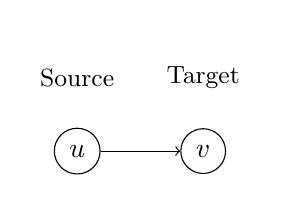
\begin{tikzpicture}[scale=0.8,every node/.style={draw=black,circle}]
		\node[label={\small Source}] (u) at (0,0) {$u$};
		\node[label={\small Target}] (v) at (2,0) {$v$};
		\draw[->] (u) to (v);
		\end{tikzpicture}
		\caption{Example of an oriented edge. By convention, $o(e)$ is the target.}
		\label{fig:orientedge}
	\end{marginfigure}
\end{defn}
\begin{defn}[Out-rooted orientation]
	An orientation of a rooted tree is called \textbf{out-rooted} if every vertex except the root is the target of exactly one edge.
\end{defn}
\begin{lem}
	For every rooted trees, there exists a unique out-rooted orientation.
\end{lem}
\begin{proof}
	Orient the edges from the root towards the neighbors of the root. Then, orient the edges from vertices at distance $i$ from the root towards the vertices at distance $j$ from the root. This is a out-rooted orientation although the proof is left to the reader. Now, we will show that this is the unique orientation. Suppose $o_1$ and $o_2$ are two out-rooted orientation of some rooted tree $T$ with a root $r$. If $|V(T)| = 1$ there are no edges so $o_1$ is vacuously equal to $o_2$. Suppose that $|V(T)| > 1$, then take a leaf $v \in V(T) \setminus \{r\}$ (we know there exists one from Lemma 39). Denote $w$ to be the only neighbor of $v$ and $e = \{u,w\}$ to be the edge that connects them. Clearly, we have $o_1(e) = o_2(e) = v$ because if $w$ was the target, $v$ would not have any incoming edge. Define $o'_1 = o_1 \vert_{E(T) \setminus \{e\}}$ and $o'_2 = o_2 \vert_{E(T) \setminus \{e\}}$. Clearly, they are out-rooted orientation of $T-v$ and by induction hypothesis, we must have $o'_1 = o'_2$. However, this must mean that $o_1 = o_2$ because we already saw that they agree on $e$ which was the only edge we removed.
\end{proof}
\begin{proof}[Proof of Cayley's formula]
	Denote $t'_n$ to be the number of rooted trees on $\{1,\dots, n\}$. There is $n$ possible choices for the root so we have $t'_n = n\cdot t_n$. Thus, we will show that $t'_n = n^{n-1}$. We already know that the number of trees on $\{1, \dots, n\}$ with an out-rooted orientation is the same as $t'_n$, so our formula does not change here. Denote $t''_n$ to be the number of trees on $\{1,\dots, n\}$ with an out-rooted orientation and an ordering of the edges. Clearly, there are $(n-1)!$ possible choices for this ordering ($|S_{n-1}|$), so we obtain $t''_n = t'_n(n-1)!$. Our goal is now to show that $t''_n = n^{n-1}(n-1)!$.
	
	We will describe a procedure to build the trees counted by $t''_n$ and then we will count the number of ways to run the procedure. The procedure will maintain two key properties : 
	\begin{itemize}
		\item Whatever is built at each step is acyclic.
		\item Every vertex will be the target of at most one edge.
	\end{itemize}
	The zeroth step is to start with an empty graph on $\{1,\dots, n\}$. The next $n-1$ steps are the following:
	\begin{enumerate}
		\item Choose a vertex $s \in \{1,\dots, n\}$
		\item Choose a vertex $t \in \{1,\dots, n\}$ such that $t \neq s$, $t$ has no incoming edge and adding the edge $\{s,t\}$ will not create a cycle.
		\item Add the edge $\{s,t\}$ with orientation $o(\{s,t\}) = t$.
	\end{enumerate}
	Notice that if the procedure is run with at least one different choice for $s$ or $t$ you get a different tree. Hence, we need to count the number of choices we have. Clearly, we always have $n$ choices for $s$. Observe that a the $k+1$th step, the graph has $n-k$ connected components. Using the invariants we can see that each of these components have exactly one vertex with no incoming edge. Since connecting two components with an edge cannot create a cycle, we have $n-k$ choices for $t$. Hence, the total number of choices is $t''_n = \prod_{k=1}^{n-1}n(n-k) = n^{n-1}(n-1)!$.
\end{proof}

\section{Spanning trees}
While trees can be studied on their own, it is sometimes useful to study trees embedded in a graph.

\begin{defn}[Forest]
	A \textbf{forest} is a graph with no cycle (also called acyclic). In other words, each connected components of $G$ are trees.
\end{defn}
\begin{defn}
	Let $G$ be a graph, a \textbf{forest in} $G$ is an acyclic subgraph of $G$.
\end{defn}
\begin{defn}[Spanning subgraph]
	Let $G= (V,E)$ be a graph, and $H$ be a subgraph of $G$. We say that $H$ is a \textbf{spanning subgraph} of $G$ if $V(H) = V$.
\end{defn}
\begin{defn}[Spanning tree]
	Let $G$ be a graph, a \textbf{spanning tree} of $G$ is a spanning subgraph of $G$ that is a tree.
\end{defn}
\begin{prop}
	If $G$ is connected, then $G$ has a spanning tree.
\end{prop}
\begin{proof}
	Let $G$ be a graph, take a connected spanning subgraph of $G$ which is minimal with respect to the number of edges. We know at least one connected spanning subgraph exists because $G$ itself satisfies these properties. Call this subgraph $T$ and we claim that it is a tree. Suppose that there exists a cycle $\{v_0, e_1, v_1, \dots, e_k, v_0\}$ in $T$. Then, $T-e_k$ is still a connected spanning subgraph of $G$ and has one less edge than $T$. We get a contradiction. 
\end{proof}
\begin{defn}[Fundamental cycle]
	Let $G$ be a graph and $T$ be a spanning tree of $G$. Moreover, take one edge $e \in E(G)\setminus E(T)$. We define the \textbf{fundamental cycle} of $G$ with respect to $T$ and $e$ to be the unique cycle in $T+e$.
\end{defn}
\begin{prop}
	In the same setting as last definition, take any edge $f$ in the fundamental cycle with respect to $T$ and $e$. Then, $T_p = (T+e)-f$ is a spanning tree.
\end{prop}
\begin{proof}
	There is only one cycle in $T+e$, by removing $f$, we clearly do not create any cycle nor disconnect the graph, hence $T_p$ is still acyclic and connected. Furthermore, we did not remove edges so $V(T_p) = V(T) = V(G)$ and we see that $T_p$ is indeed spanning.
\end{proof}
One meaningful problem related to spanning trees is the minimum spanning tree problem which is well studied in computer science and especially in algorithm design. We have one definition to make before stating the problem.
\begin{defn}[Weighted graph]
	A \textbf{weighted graph} is a triple $(V,E,w)$ where $(V,E)$ is a graph and $w: E \rightarrow \R$ assigns weights to each edge. For any subgraph $H$ of a weighted graph $G$, $w(H) = \sum_{e \in E(H)}w(e)$ is the weight of $H$.
\end{defn}
The minimum spanning tree problem or MST for short asks what is the spanning tree with smallest weight for some connected weighted graph $G$. We will give an algorithm to find the MST of such a graph. The input of this algorithm is a weighted graph and the output is a spanning tree of this graph with minimal weight.

Denote the input $G=(V,E,w)$. The first step of the algorithm is to initialize $T = (V,\emptyset)$. Then, we sort the edges in $E$ according to their weight to obtain an ordering $\{e_1, \dots, e_m\}$ with $w(e_i) < w(e_j)$ for all $i < j$. Next, we iterate from $i=1$ to $i=m$. At each iteration, we add $e_i$ to the edges of of $T$ if $T+e_i$ is still a tree. At the end of these iteration, we will obtain a MST of $G$. It is clear that $T$ is a spanning tree but it is maybe not so clear that it is minimal. What follows is the proof of that.

\begin{proof}[Correctness of Kruskal's algorithm]
	We will prove it by induction on the number of edges of $T$. At the start when $T$ has no edges, there clearly exists a MST of $G$ which contains $T$. We will show that this property holds whenever $T$ gets a new edge implying that the final $T$ is a MST of $G$. Suppose that at some step in the algorithm, we are about to add some edge $e$ to $T$ and that $M$ is a minimal spanning tree containing $T$. If $e$ is in $M$, then clearly $M$ contains $T+e$. If $e$ is not in $M$, then $M+e$ has a cycle. Moreover, there exists an edge $f$ in the cycle and not in $T$ (if there were no such edge, $e$ would have created a cycle in $T$). We obtain that $M-f+e$ is a spanning tree, this means that its weight is no less that the weight of $M$ because $M$ is a MST. In addition, $w(f) < w(e)$ is not possible or the algorithm would have chosen to add $f$ before $e$. Hence, we must have $w(f) = w(e)$ and $M-f+e$ is in fact a MST containing $T$.
\end{proof}

We now explore a problem that is closely related to the MST problem. In a simple graph, how can you find the shortest path between two vertices ? If we consider an unweighted graph, the solution is pretty simple. Run a breadth-first search algorithm on the graph starting at the source vertex and stop when the target vertex is reached for the first time. The path taken to the target vertex must be of shortest length. Next, we answer the same question in the setting of a weighted graph but we give a definition first.

\begin{defn}[Distance in a graph]
	Let $G = (V,E,w)$ be a weighted graph with $w : E \rightarrow \R^{+}$. Define the function of \textbf{distance} in $G$ like so :
	$$ \dist_G : V \times V \rightarrow \R^{+}, (u,v) \mapsto \min_{P \in \{\mbox{paths from u to v}\}} w(P)$$
\end{defn}
\begin{rem}
	We a require that the weights are positive because it is extremely hard to solve the question otherwise and most real life settings only need positive weights. Also, note that in the MST problem, we said that the image of $w$ was in the reals but it is sufficient for it to be in a linearly ordered set.
\end{rem}
\begin{prop}
	The distance function in a weighted graph is a metric.
\end{prop}
\begin{proof}
	Not in the scope of this class.
\end{proof}

Once again, we present an algorithm that will find the shortest path between two vertices in a graph. Without loss of generality, we assume that this graph is connected. Let $G = (V,E,w)$ be a connected weighted graph, we want to find the shortest path between $s$ and $t$, both in vertices in $V$.

We describe Dijkstra's algorithm. This algorithm will build a tree $T_s$ such that $\forall v \in T_s$, $\dist_G(s,v) = \dist_{T_s}(s,v)$. In particular, the unique path in $T_s$ from $s$ to $t$, will be a shortest path in $G$. Each step of the algorithm will add one edge to $T_s$. Note that since we will stop when $t$ is reached, $T_s$ is not necessarily a spanning tree. 

In step 0, the tree is initialized to $T_s^0 = (\{s\},\emptyset)$. Next, we repeat this step while $t \notin V(T_s^k)$. Choose an edge $f = \{u,v\} \in E$ such that $u \in T_s^{k-1}$, $v \notin T_s^{k-1}$ and $\dist_{T_s^{k-1}}(s,u) + w(f)$ is minimal. Add the edge $f$ to get $T_s^k = T_s^{k-1}+f$.

\begin{proof}[Correctness of Dijkstra's algorithm]
In order to prove that this algorithm achieves the result we want, we will show that the following invariant holds at any step $k$ : $$\forall v \in T_s^k, \dist_{T_s^{k}}(s,v) = \dist_G(s,v)$$
When $k=0$, this is clearly true since the distance from a vertex to itself is 0. Let $k>0$ and assume that this invariant holds for all the steps before $k$. Call $v$ the new vertex added at step $k$, namely, $v \in T_s^k\setminus T_s^{k-1}$. Denote $f = \{x,v\}$ to be the edge that was added at this step. We claim that for any path $P = \{u_0,e_1,u_1,\dots, e_l,u_l\}$ with $u_0 = s$ and $u_l = v$, $w(P) \geq \dist_{T_s^k}(s,v)$. Let $u_j$ be the first vertex in $P$ that is not in $T_s^{k-1}$, we know it exists since $v \notin T_s^{k-1}$. We obtain the following:
\begin{align*}
	w(P) &\geq \dist_G(s,u_{j-1}) + \sum_{i=j}^l w(e_i)\\
	&\geq \dist_G(s,u_{j-1}) + w(e_j)\\
	&\geq \dist_{T_s^{k-1}}(s,u_{j-1}) + w(e_j) && \mbox{By induction hypothesis}\\
	&\geq \dist_{T_s^{k-1}}(s,x) + w(f)&& \mbox{By the steps in the algorithm}\\
	&= \dist_{T_s^{k}}(s,v)
\end{align*}
\end{proof}
\section{Euler tours}
In this section, we will talk about multigraphs. The arguments we will make are valid for graphs as well but they require some details which we do not want to spend too much time on. We start with some simple definitions.

\begin{defn}[Tour]
	A \textbf{tour} in $G$ is a walk $\{v_0, e_1, v_1, \dots, e_k, v_k\}$ such that $\forall i\neq j, e_i \neq e_j$.
\end{defn}
\begin{defn}[Closed walk/tour]
	A walk/tour is said to be \textbf{closed} if $v_0 = v_k$, namely, the start and end vertex is the same.
\end{defn}
\begin{defn}[Eulerian tour]
	A tour is said to be \textbf{Eulerian} if $E(G) = \{e_1, \dots, e_k\}$ and $V(G) = \{v_1,\dots, v_k\}$.
\end{defn}

We would like to find some necessary and sufficient condition for a graph to contain an Eulerian tour. You can try to draw some graphs and figure out a condition but you might remember from the K\"onigsberg bridges problem that you should have at most two vertices of odd degree for a graph to contain an Eulerian tour. We state a stronger statement and prove our result as a corollary.

\begin{thm}
	A multigraph $G$ contains a closed Eulerian tour if and only if $G$ is connected and there is no vertices of odd degree.
\end{thm}
\begin{cor}
	A multigraph $G$ contains an Eulerian tour if and only if it is connected and contains at most two vertices of odd degree.
\end{cor}
\begin{proof}[Proof of corollary]
	($\Rightarrow$) This direction does not use the theorem. If there is an Eulerian tour, then all the vertices of $G$ are in the same walk and so $G$ must be connected. Moreover, all the vertices which are not the endpoints of the walk must have even degree and we have at most two distinct endpoints so we are done.
	
	($\Leftarrow$) If the number of vertices of odd degree is 0, we can use the theorem. There cannot be only one vertex of odd degree so the case where there is two vertices of odd degree is the only one left. Call $u,w$ the vertices with odd degree. Let $G' = G+\{u,w\}$\footnote{This is where having a multigraph is useful since we do not need to handle the case where the edge is already there}, we can now use the theorem to find a closed Eulerian tour $T = \{v_0, e_1, \dots, e_i, v_i, \dots, e_k, v_k\}$ where, without loss of generality, $v_0 = v_k = u$ and $e_i = \{u,w\}$. Define the sub-walks $T_1 = \{v_0, e_1, \dots, v_{i-1}\}$ and $T_2 = \{v_i, \dots, e_k, v_k\}$. Clearly, $T_1$ and $T_2$ are walks in $G$, and $T_2T_1$ is an Eulerian tour in $G$.
\end{proof}
\begin{proof}[Proof of theorem]
	($\Rightarrow$) As in the corollary, $G$ is connected and all the vertices which are not endpoints of $T$ have even degree. Moreover, since the start and endpoint is the same, it must have even degree as well.
	
	($\Leftarrow$) Let $T = \{v_0, e_1, \dots, e_k,v_k\}$ be the longest tour in $G$ (with respect to the number of edges), we claim that $T$ is closed and Eulerian.
	
	First, assume towards a contradiction that $T$ is not closed. Look at the graph $H=(V,E(T))$. The vertices $v_0$ and $v_k$ must have odd degrees in $H$ since $v_0 \neq v_k$. Since we know $\deg(v_0)$ is even in $G$, there exists an edge $f =\{v_0,x\} \in E(G)\setminus E(T)$. Clearly, $xfT$ is a tour with more edges than $T$, so we obtain that $T$ must be closed. 
	
	Next, assume towards a contradiction that there exists an edge $f=\{u,w\} \in E(G)\setminus E(T)$. We consider two cases. If at least one vertex of $f$ is somewhere in $T$, without loss of generality, $u = v_i$ for some $0 \leq i \leq k$, define the sub-walks $T_1 = \{v_0, e_1, \cdots, v_{i-1}\}$ and $T_2 = \{v_i, \dots, v_k\}$. We can see that $T' = v_iT_2v_kT_1v_ifw$ is a longer tour so we get a contradiction. Conversely, if $f$ has no endpoint in $T$. Let $P$ be the shortest path from some vertex in $T$ to some vertex not in $T$. Clearly, $P$ is just an edge $\{x,y\}$ with $x \in V(T)$ and $y \notin T$ and this leads to a contradiction like in the first part of this proof. Since all the edges are in $T$ and $G$ is connected, all the vertices must also be in $T$ so $T$ is Eulerian.
\end{proof}

A notion related to Eulerian tours is Hamiltonian paths.

\begin{defn}[Hamiltonian paths]
	A path is said to be \textbf{Hamiltonian} if it visits all vertices.
\end{defn}
\begin{defn}[Hamiltonian cycle]
	A Hamiltonian path with its starting point being its endpoint is called a \textbf{Hamiltonian cycle}.
\end{defn}
Unfortunately, as of today, there is no necessary and sufficient condition for a graph to contain a Hamiltonian cycle. However, there is a sufficient condition.
\begin{thm}[Ore's theorem]
	Let $G = (V,E)$ be a graph with $n = |V| \geq 3$. Suppose that for every pair $u,w \in V$ such that $\{u,w\} \notin E$, $\deg(u) + \deg(w) \geq n$, then $G$ contains a Hamiltonian cycle.
\end{thm}
\begin{proof}
	Fix $n$, the number of vertices, we will prove this by induction on the number of edges missing from $K_n$, namely, an induction on $z = \binom{n}{2}-|E|$. When $z=0$, the graph is $K_n$ which clearly contains a Hamiltonian cycle. Let $z > 0$ and assume that any graph with $z-1$ edges removed that satisfies the property in the theorem contains a Hamiltonian cycle. Then, consider a graph $G$ with $z$ edges removed, still satisfying the property. We know there exists an edge $e = \{u,w\} \notin E(G)$. Consider the graph, $H = G+e$, it is trivial to show that $H$ also satisfies the property and has $z-1$ edges removed, so by our induction hypothesis, it contains a Hamiltonian cycle $C_H$. If $C_H$ does not contain the edge $e$, we are done since $C_H$ is also a Hamiltonian cycle in $G$. On the other hand, if $C_H$ contains $e$, then, we can write $C_H = \{v_1, e_1, v_2, \dots, v_n, e, u\}$ where $v_0 = u$ and $v_n = w$.
	
	We claim that there exists an integer $i \in \{3,\dots, n-1\}$ such that $v_1$ is adjacent to $v_i$ and $v_n$ is adjacent to $v_{i-1}$. First, denote $U = N_G(u)$ to be the neighbors of $u$ in $G$, clearly , $U \subseteq \{v_2, \dots, v_{n-1}\}$. Also, denote $N_G(w)$ to be the neighbors in $G$, we can infer that $N_G(w) \subseteq \{v_2, \dots, v_{n-1}\}$. Lastly, we define $W = \{v_{i+1} \mid v_i \in N_G(w)\} \subseteq \{v_3, \dots, v_n\}$. Notice that $|U| = \deg(u)$ and $|W| = \deg(w)$, so $|U| + |W| \geq n$ by our assumption that $G$ satisfies the property. However, we also know that $|U \cup W| \leq n-1$ because $v-1 \notin U\cup W$, hence we must have $U \cap W \neq \emptyset$. This proves our claim that there exists $i \in \{3,\dots, n-1\}$ such that $v_i \in U \cap W$, namely, $v_1 = u$ is connected to $v_i$ and $v_n = w$ is connected to $v_{i-1}$.
	
	Using our claim, we can construct a Hamiltonian cycle in $G$. It is really easier to see it in a diagram but here is the construction. Let $P_1$ be the path from $u$ to $v_{i-1}$ in $C_H$, $P_2$ be the path from $w$ to $v_{i}$ in $C_H$ and denote $e_1 = \{u,v_i\}$ and $e_2 = \{w,v_{i-1}\}$. We construct $C_G = P_1e_2P_2e_1$, one can verify that this is indeed a Hamiltonian path in $G$.
\end{proof}
\begin{cor}
	Let $G = (V,E)$ be a graph, then $\min_{v \in V} \deg(v) \geq \frac{n}{2}$ implies that $G$ contains a Hamiltonian cycle.
\end{cor}
We state this really simple corollary, because we will introduce the next section with an example to show that the bound is tight. 
\begin{exmp}
	Let $A$ be an empty graph on $a$ vertices and $B$ be an empty graph on $a+1$ vertices. Connect all the vertices in $A$ to all the vertices in $B$ with an edge. We have $\deg(v) \geq a$ for all vertices but $a < \frac{2a+1}{2}$, so we want to show that there is no Hamiltonian cycle. Indeed, any cycle must visit the same number of vertices in $A$ and $B$ but it cannot do that if it visits all vertices. The kind of graph we described is the subject of the next section.
\end{exmp}

\section{Bipartite graphs}
\begin{defn}[Bipartite graph]
	We say that a graph $G$ is \textbf{bipartite} if there exists sets $A, B \subseteq V(G)$ such that $A \cup B = V$, $A \cap B = \emptyset$ and $\forall e \in E(G), |e \cap A| = |e \cap B| = 1$.
\end{defn}
\begin{exmps}
	Paths and cycles of even length are bipartite. Indeed, we already know that we can 2-color them, then we can have each color correspond to a set of the bipartition. It is also easy to show that trees are bipartite \footnote{Pick a root in the tree and consider the vertices of even distance to the root and odd distance to the root}. Moreover, subgraphs of bipartite graphs are clearly bipartite. In particular, if a graph contains a subgraph that is not bipartite, then the graph cannot be bipartite.
\end{exmps}
The next theorem gives a necessary and sufficient condition for a graph to be bipartite.
\begin{thm}
	A graph $G$ is bipartite if and only if it has no odd cycle.
\end{thm}
We stated this theorem first because it is the result we will most likely use when trying to say if a graph is bipartite but we will prove it with an intermediary step.
\begin{thm}
	Let $G = (V,E)$ be a graph, then the following are equivalent :
	\begin{enumerate}
		\item $G$ is bipartite
		\item $G$ does not contain a closed walk of odd length
		\item $G$ does not contain an odd cycle
	\end{enumerate}
\end{thm}
\begin{proof} We will denote $A$ and $B$ to be the sets of the bipartition of $G$.

	($1 \implies 2$) Pick any closed walk $W = \{v_0, e_1, v_1, \dots, e_m, v_m\}$. Without loss of generality, assume $v_0 = v_m \in A$. Each edge in $W$ goes from $A$ to $B$ or from $B$ to $A$, since the start and end of the walk are in $A$, there must be an even number of edges in $W$.
	
	($2 \implies 1$) The contrapositive of this statement follows immediately from the definition because an odd cycle is a closed walk of odd length.
	
	($3 \implies 1$) Without loss of generality, assume that $G$ is connected and let $T$ be any spanning tree of $G$. Let $u \in V$ and define the following bipartition for $T$ : \begin{align*}
		A' &= \{v \in V \mid \dist_T(u,v) \equiv 0 \Mod{2}\}\\ 
		B' &= \{v \in V \mid \dist_T(u,v) \equiv 1 \Mod{2}\}
	\end{align*}
	It is left to prove that for any $e \in E(G) \setminus E(T)$, $|e \cap A'| = |e \cap B'| = 1$. Assume towards a contradiction and without loss of generality that for some $e = \{v_1, v_2\}$, we have $v_1, v_2 \in A'$. Denote $C_e$ to be the fundamental cycle of $e$ in $T$. The path $P$ which is the cycle $C_e$ with the edge $e$ removed has both its endpoints in $A$ so it must have even length. Thus, $C_e$ is an odd cycle and we get a contradiction.
\end{proof}
\begin{prop}
	Let $G$ be a simple graph. $G$ is bipartite if and only if it contains no induced cycle of odd length.
\end{prop}
\begin{proof}
	($\Rightarrow$) $G$ is bipartite so it contains no odd cycle, in particular, none of its induced subgraph can be a cycle of odd length.
	
	($\Leftarrow$) We prove the contrapositive. Suppose there is an odd cycle, then take one with shortest length, call it $C = \{v_0,e_1,\dots, e_k,v_k\}$ where $v_0 = v_k$. If the subgraph induced by the vertices on this cycle is not a cycle, then $\exists i<j, |j-i| > 1, \{v_i, v_j\} \in E(G)$. This edge breaks $C$ into two cycles, and one must be of odd length and smaller than $C$. This contradicts our choice of $C$.
\end{proof}
\section{Matching in graphs}
\begin{defn}[Matching]
	Let $G = (V,E)$ be a graph. A \textbf{matching} in $G$ is a set of edges $M \subseteq E$ with the property that every vertex in $V$ is incident to at most one edge in $M$. A matching is said to be \textbf{perfect} if all vertices are incident to exactly one edge in $M$.
\end{defn}
A observation one can make fairly quickly is that for a matching $M$ in $G$, we have $|M| \leq \lfloor \frac{|V|}{2}\rfloor$. Looking at this bound, one could ask how to find the largest matching in $G$. Before reaching for that goal, we introduce related notions.
\begin{defn}[2-factor]
	Let $G = (V,E)$ be a graph, a \textbf{2-factor} in $G$ is a set of edges $F \subseteq E$  with the property that every vertex in $V$ is incident to exactly two edges in $F$.
\end{defn}
\begin{exmp}
	If a graph contains a Hamiltonian cycle $H$, the set edges of $H$ is a 2-factor in $G$.
\end{exmp}
\begin{defn}[$k$-regularity]
	A graph $G=(V,E)$ is said to be \textbf{$k$-regular} if $\forall v \in V,\deg(v) = k$.
\end{defn}
\begin{prop}
	For any $k\geq 1$, a $(2^k)$-regular graph contains a 2-factor.
\end{prop}
\begin{proof}
	Without loss of generality, we will assume that $G$ is connected and we will prove it by induction. For $k=1$, every vertex is incident to exactly two edges in the graph so the set of all edges is a 2-factor. Assume that the proposition is true for some $k\geq 1$, then let $G$ be a $(2^{k+1})$-regular graph which is (without loss of generality) connected. Since the degree of all vertices is even, we know that there exists a closed Eulerian tour $T = \{v_0, e_1, \dots, e_m, v_m\}$ where $v_0 = v_m$ and $m = |E| = 2^kn$. Since $m$ is even, we can separate the set of edges like so :
	$$ E_1 = \{e_{2k} \mid k \leq \frac{m}{2}\} \quad \quad E_2 = \{e_{2k+1} \mid k < \frac{m}{2}\}$$
	Define the subgraphs $H_1 = (V,E_1)$ and $H_2 = (V,E_2)$. Observe that in the tour, each vertex is connected to the same number of edges in $E_1$ and $E_2$, so we infer that $\deg_{H_1}(v) = \deg_{H_2} = 2^k$. We can use the induction hypothesis to find two 2-factors for $H_1$ and $H_2$, clearly, the union of these 2-factors is a 2-factor for $G$.
\end{proof}
We now go back to study matchings and we will see later why the notion of 2-factors was introduced.
\begin{defn}[$M$-alternating path]
	Let $G=(V,E)$ be a graph and $M$ be a matching in $G$. An \textbf{$M$-alternating path} is a path in $G$ which alternates between edges in $M$ and edges in $E\setminus M$. Equivalently, every internal vertex in the path is connected to his neighbors in the path by one edge in $M$ and one edge in $E \setminus M$
\end{defn}
\begin{defn}[$M$-augmenting path]
	An \textbf{$M$-augmenting path} is an $M$-alternating path of non-zero length which starts in a vertex $v$ not incident to any edge in $M$ and ends in a vertex $w \neq v$ not incident to any edge in $M$.
\end{defn}
\begin{lem}[Berge]
	Let $G = (V,E)$ be a graph and $M$ be a matching in $G$. $M$ is maximum matching if and only if there is no $M$-augmenting paths.
\end{lem}
\begin{proof}
	($\Rightarrow$) Assume towards a contradiction that $G$ contains an $M$-augmenting path $P$. The set $(E(P) \setminus M) \cup (M \setminus E(P))$ is a matching since every vertex outside the path is still matched by the same edge and every vertex in the path gets matched with the unique edge not in $M$ and incident to it in $P$. It also has more edges than $M$ since $P$ has more edges not in $M$ than edges in $M$.
	
	($\Leftarrow$) We will prove this direction by contrapositive, namely, we will show that if $M$ is not maximal, then there exists a $M$-augmenting path. We know that there exists a larger matching $M'$, so we define $H = (V, M \cup M')$. We know that $\forall v \in V, \deg_H(v) \leq 2$, so $H$ is the union of cycles and paths.
	
	We have two claims that imply that there exists an $M$-augmenting. The first one is that all cycles in $H$ have even length. Indeed, for each cycle $C$ in $H$, each vertex must be connected to one edge in $M\setminus M'$ and one edge in $M'\setminus M$ and this cannot happen if there is an odd amount of edges. The second claim that there is a connected component with more edges in $M'$ than $M$ follows from the fact that $|M'| > |M|$. This component must be a path because of our first claim and this implies that this path is $M$-augmenting.
\end{proof}

In bipartite graphs, the problem of finding maximal matching is simpler and it also uses the concept of a vertex cover.

\begin{defn}[Vertex cover]
	A \textbf{vertex cover} in a graph $G = (V,E)$ is a set of vertices $X \subseteq V$ such that any edges are incident to at least one vertex in $X$.
\end{defn}
\begin{defn}[Sizes of minimal cover and maximal matching]
	Let $G$ be a graph, we will denote the size of a minimal vertex cover with $\tau(G)$ and the size of a maximal matching with $\nu(G)$.
\end{defn}
\begin{rem}
	We can see that $\nu(G) \leq \tau(G)$ since we need at least one vertex per edge in the maximal matching in order to cover all edges. Also, we have $\tau(G) \leq 2\nu(G)$ because the set of all endpoints of the edges in the maximal matching covers all the edges. Moreover, one can find via simple graph examples that these inequalities are tight.
\end{rem}
\begin{thm}[Konig]
	Let $G$ be a bipartite graph, then $\tau(G) = \nu(G)$.
\end{thm}
\begin{proof}
	It is immediate that $\tau(G) \leq \nu(G)$ since for a maximum matching $M$, the vertex cover should contain at least one endpoint for each edge. Next, we show that $\nu(G) \leq \tau(G)$. Let $A$ and $B$ be the bipartition of $G$ and $M$ be a matching of size $\nu(G)$. Denote $A = A_M \cup A_N$ and $B= B_M \cup B_N$ where $A_m$ and $B_M$ are the vertices, in $A$ and $B$ respectively, that are matched by $M$ and $A_N = A \setminus A_M$ and $B_N = B \setminus B_M$. Further decompose this sets in $A_M = A_X \cup A_Z$ and $B_M = B_X \cup B_Z$ with the following definitions :
	\begin{align*}
		A_Z &= \{ a \in A_M \mid \exists M\mbox{-alternating path starting in } A_N \mbox{ and ending in } a\}\\
		B_Z &= \{b \in B_M \mid \exists a \in A_Z, \{a,b\} \in M\}\\
		A_X &= A_M \setminus A_Z \quad \quad B_X = B_M \setminus B_Z
	\end{align*}
	Next, we will make some simple observations that will lead us to find a good vertex cover.
	\begin{itemize}
		\item There is no edge in $G$ between $A_N$ and $B_N$. If it were the case, this edge could be added to $M$ contradicting the maximality of $M$.
		\item There is no edge in $G$ between $A_N$ and $B_X$. If it were the case, we would have an $M$-alternating path of length two going from $A_N$ to $B_X$ then to $A_X$. This implies the vertex where this path ends in $A_X$ should be in $A_Z$ by definition.
		\item There is no edge in $G$ between $B_N$ and $A_Z$. If it were the case, we could glue this edge to the $M$-alternating path starting in $A_N$ and ending in the vertex in $A_Z$, yielding an $M$-augmenting path and contradicting Berge's lemma.
		\item There is no edges in $G$ between $A_Z$ and $B_X$. If it were the case we could glue that edge and and edge in $M$ from $B_X$ to $A_X$ to the $M$-alternating path starting in $A_N$ and ending in the vertex in $A_Z$ to form an $M$-alternating path from $A_N$ to $A_X$, which contradicts the definition.
	\end{itemize}
\begin{marginfigure}
	\begin{center}
		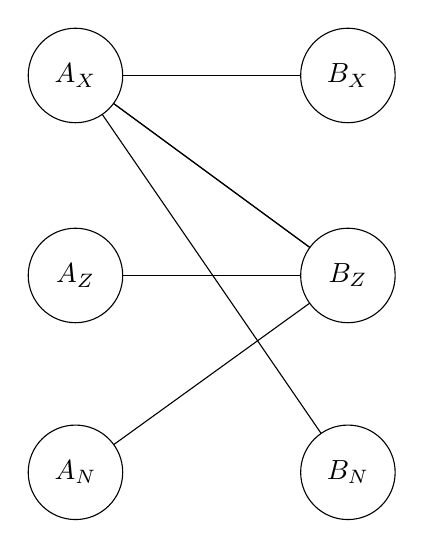
\begin{tikzpicture}[scale=0.2]
		\tikzstyle{every node}+=[inner sep=0pt]
		\draw [black] (11.1,-7) circle (3);
		\draw (11.1,-7) node {$A_X$};
		\draw [black] (11.1,-19.7) circle (3);
		\draw (11.1,-19.7) node {$A_Z$};
		\draw [black] (11.1,-32.2) circle (3);
		\draw (11.1,-32.2) node {$A_N$};
		\draw [black] (28.4,-7) circle (3);
		\draw (28.4,-7) node {$B_X$};
		\draw [black] (28.4,-19.7) circle (3);
		\draw (28.4,-19.7) node {$B_Z$};
		\draw [black] (28.4,-32.2) circle (3);
		\draw (28.4,-32.2) node {$B_N$};
		\draw [black] (14.1,-7) -- (25.4,-7);
		\draw [black] (13.52,-8.78) -- (25.98,-17.92);
		\draw [black] (12.8,-9.47) -- (26.7,-29.73);
		\draw [black] (25.98,-17.92) -- (13.52,-8.78);
		\draw [black] (25.4,-19.7) -- (14.1,-19.7);
		\draw [black] (25.97,-21.46) -- (13.53,-30.44);
		\end{tikzpicture}
	\end{center}
\caption{Summary of the observations in Konig's theorem}
\label{fig:konigproof}
\end{marginfigure}
	Figure \ref{fig:konigproof} shows a graph that summarizes the observations by showing the edges in the graph that can be there. From here, we clearly see that $S = A_X \cup B_Z$ is a vertex cover. We can compute its size like so $$|S| = |A_X| + |B_Z| = |A_X| + |A_Z| = |A_M| = |M|$$
	implying that $\nu(G) \geq \tau(G)$.
\end{proof}
\begin{defn}[Matching covering sets]
	Let $A \subseteq V(G)$. An \textbf{$A$-covering} matching $M$ is a matching $M$ in $G$ with the property that every vertex in $A$ is incident to an edge in $M$.
\end{defn}
\begin{defn}[Neighbors notation]
	Let $G$ be a graph, $v \in V(G)$ and $S \subseteq V(G)$. We denote the set of \textbf{neighbors} of $v$ as $N(v)$ and $N(S)$ denotes the union over $v \in S$ of $N(v)$.
\end{defn}
\begin{thm}[Hall]
	Let $G$ be a bipartite graph with bipartition $A$ and $B$, then there exists an $A$-covering matching in $G$ if and only if $\forall S \subseteq A, |N(S)| \geq |S|$.
\end{thm}
\begin{proof}
	($\Rightarrow$) Follows trivially from the pigeonhole principle.
	
	($\Leftarrow$) Since we are looking for an $A$-covering matching and a vertex covering cannot be larger than one part of $G$. It is enough to show that $\nu(G) = |A|$ which is equivalent to $\tau(G)=|A|$ by Konig's theorem. Let $X$ be a vertex cover in $G$. Denote $A' =  A \setminus X$. By our hypothesis, $|N(A')| \geq |A'|$ and since $N(A') \subseteq B \cap X$, we get $|A|= |A \cap X| + |A'| \leq |A \cap X| + |B \cap X| = |X|$. Since $|A| \leq |X|$ and $A$ is a vertex cover, we have $\nu(G) = |A|$.
\end{proof}

\begin{cor}
	A $d$-regular graph bipartite contains a perfect matching.
\end{cor}
\begin{proof}
	Let $A$ and $B$ be the bipartition of this graph. In order to find a perfect matching, we first need $|A| = |B|$. This is true because the number of edges leaving $A$ and leaving $B$ is the same, so we have $|A|\cdot d = |B| \cdot d$. Now, we only have to show Hall's condition holds for $A$ to get an $A$-covering matching which will be perfect. Let $S \subseteq A$, the number of edges leaving $S$ is less than the number of edges leaving $N(S)$ so we get $d\cdot |S| \leq d \cdot |N(S)|$ implying Hall's condition is true. 
\end{proof}
\begin{cor}
	Every $(2k)$-regular graph has a 2-factor.
\end{cor}
\begin{proof}
	Since every vertex has an even degree, $G$ contains an Eulerian tour. Moreover, each vertices has $k$ incoming edges and $k$ outgoing edges in that tour. Split up each vertex into $v_i$ and $v_o$ connected to the incoming edges and outgoing edges respectively. This yields a $k$-regular bipartite graph so it contains a perfect matching. This matching corresponds to a 2-factor in the original graph since $v_i$ and $v_o$ both have degree 1 in that matching.
\end{proof}
\begin{cor}
	Every $(2k)$-regular graph has $k$ disjoint 2-factors.
\end{cor}
We have enough results on bipartite graphs so let us move back to matchings in general graphs.

\begin{defn}[Independent sets]
	Let $G = (V,E)$ be a graph. A subset of vertices $X$ is said to be \textbf{independent} if the induced subgraph $G[X]$ has no edges. We will use $\alpha(G)$ to denote the maximal size of an independent set in $G$.
\end{defn}
\begin{prop}
	Let $G=(V,E)$ be any graph, $\alpha(G) + \tau(G) = |V|$.
\end{prop}
\begin{proof}
	We first show that $\alpha(G) \geq |V| - \tau(G)$. Let $C \subseteq V$ be a minimum vertex cover and let $X = V \setminus C$. $X$ is an independent set because if there is an edge completely in $X$, this means $C$ does not cover it.
	
	Then, we show that $\tau(G) \leq |V| - \alpha(G)$. Let $X \subseteq V$ be an independent set of size $\alpha(G)$ and let $C = V \setminus X$. $C$ is a vertex cover because if an edge has no endpoints in $C$, it must be completely in $X$ contradicting its independence.
	
	Using the two inequalities, we obtain $\alpha(G) + \tau(G) = |V|$.
\end{proof}
\begin{defn}[Edge cover]
	Let $G$ be a graph without isolated points (i.e: $\forall v \in V, \deg(v) > 0$). We say that $L \subseteq E$ is an \textbf{edge cover} if every vertex is incident to at least one edge in $L$. We use $\rho(G)$ to denote the minimum size of an edge cover.
\end{defn}
\begin{prop}[Gallai]
	Let $G=(V,E)$ be any graph, $\rho(G) + \nu(G) = |V|$.
\end{prop}
\begin{proof}
	We first prove that $\rho(G) \leq |V| - \nu(G)$. Let $M$ be a maximum matching in $G$ and define $L = M \cup Z$ where $Z$ is a set containing one incident edge for each vertex not matched by $M$. Note that $|Z| = |V| - 2|M|$ there are $2|M|$ vertices matched by $M$ and each edge chosen in $Z$ cannot be chosen twice. This gives $|L| = |M| + |Z| = |V| -|M| = |V| - \nu(G)$. Since $L$ is an edge cover, the inequality must hold.
	
	Then, we show that $\nu(G) \geq |V| - \rho(G)$. Let $L$ be an edge cover of minimal size. Denote $H \subseteq G = (V,L)$. We claim that for each edge $e \in L$ there is at least one of its endpoint $v$ with $\deg_H(v) = 1$. Assume otherwise, both endpoint have a degree higher than one so we can remove $e$ from $L$ and still get a cover, contradicting the minimality of $L$. We can conclude that $H$ is acyclic, or equivalently, it is a forest. Recall that $|V(H)| - |E(H)| = \comp(H)$. Moreover, no component of $G$ is of size one since $L$ is an edge cover. Choosing one edge in each component clearly defines a matching in $G$ of size $\comp(H) = |V| - \rho(G)$.
	
	Using the two inequalities, we obtain $\rho(G) + \nu(G) = |V|$.
\end{proof}
\begin{cor}
If $G$ is bipartite, $\alpha(G) = \rho(G)$.
\end{cor}

We will now try to find something similar to Hall's theorem in general graphs. Namely, we would like to find a necessary and sufficient condition to find a perfect matching in $G$. We first observe that $|V|$ being even is already a necessary condition, but it is not sufficient. We will look at a more general condition but with the same idea behind. Before that we state a simple vocabulary definition.

\begin{defn}[Odd components]
	Let $G$ be a graph, and $G_1, \dots, G_k$ be its connected components. We say that some component $G_i$ is \textbf{odd} if $|V(G_i)|$ is odd. Moreover, we use $\odd(G)$ to denote the number of odd components of $G$.
\end{defn}
\begin{thm}[Tutte]
	Let $G = (V,E)$ be any graph, then $G$ has a perfect matching if and only if for any subset of vertices $X$, $\odd(G-X) \leq |X|$.
\end{thm}
\begin{proof}
	($\Rightarrow$) This is the trivial implication.
\end{proof}
Before giving the proof of the other implication, we will explore multiple uses for it to familiarize ourself with its consequences. The first corollary is Petersen's theorem.
\begin{thm}[Petersen]
	All 3-regular graphs containing no cut-edges have perfect matchings.
\end{thm}
\begin{cor}
	A 3-regular graph $G$ has a perfect matching if and only if it has a 2-factor.
\end{cor}
\begin{proof}
	Let $M$ be a perfect matching in $G$, $G-M$ is 2-regular so $E(G) \setminus M$ is a 2-factor. Let $F$ be a 2-factor in $G$, $G-F$ is 1-regular so $E(G) \setminus E(F)$ is a perfect matching.
\end{proof}
\begin{proof}[Proof of Petersen's theorem]
	Let $G= (V,E)$ be a 3-regular graph containing no cut-edges. It is enough to show Petersen's condition is satisfied. Without loss of generality, we assume that $G$ is connected. For $X = \emptyset$, we need to check that $|V|$ is even. By the handshaking lemma, $3|V|$ is even so $|V|$ must be even. Assume towards a contradiction that $\exists X \subseteq V$ with $|X| > 0$ and $\odd(G-X) > |X|$. We claim that each odd connected component of $G$ sends at least three edges to $X$. This would imply that $X$ has more edges than $3|X|$ contradicting the regularity of $G$.
	
	In order to prove the claim, we consider multiple cases. Denote $n$ to be the number of edges sent from some connected component $C$ to $X$. Clearly, $n \geq 1$ because the initial graph $G$ is connected. If $n=1$, the unique edge sent must be a cut-edge contradicting our hypothesis. If $n=2$, then, since $\forall v \in C, \deg_G(v) = 3$, we get $\sum_{v \in C} \deg_C(v) = 3|C| -2$ which cannot be an even number, contradicting the handshaking lemma. Therefore, we can only have $n\geq 3$. 
\end{proof}
Next, we will show that Tutte's theorem implies one direction of Hall's theorem. We will use the following observation in this proof.
\begin{lem}
	Let $G = (V,E)$ be a graph with $|V|$ even. Then for any $X \subseteq V$, $\odd(G-X) \equiv |X| \mod{2}$. We will refer to this as the parity observation.
\end{lem}
\begin{cor}
	Let $G = (V,E)$ be a bipartite graph with parts $A$ and $B$. Suppose that $\forall S \subseteq A, |N_G(S)| \geq |S|$, then $G$ has an $A$-covering matching.
\end{cor}
\begin{proof}
	Define $E' = \{\{b_1,b_2\} \mid b_1, b_2 \in B\}$ (i.e: all the edges between vertices in $B$) and define a new graph as follows:
	\[ G' = \begin{cases}
		(V, E \cup E') & |V| \text{ even}\\
		(V \cup \{b'\}, E \cup E' \cup \{\{b',b\} \mid b \in B\}) & |V| \text{ odd}
	\end{cases} \]
	This transforms the graph $G$ by adding a new vertex to $B$ if $|V|$ is odd and putting all the edges in $B$. Observe that a perfect matching in $G'$ is an $A$-covering matching in $G$. Hence, we will check Tutte's condition, namely that for any $X \subseteq V(G')$, $\odd(G'-X) \leq |X|$. If we look at the components of $G'-X$, we see that one component has the vertices in $B'-X$\footnote{$B' = B \cup \{b'\}$ if $b'$ was added, $B'=B$ otherwise} and the vertices in $A$ connected to it and all the other components only have isolated vertices of $A$. We will call the set of these isolated vertices $Y$. We know that $\odd(G'-X) \leq |Y| + 1$. Now, if we show that $|X| \geq |Y|$, we will have $\odd(G'-X) \leq |X| +1$, but by the parity observation, this is equivalent to $\odd(G'-X) \leq |X|$.
	
	In order to prove $|X| \geq |Y|$, we will show a tighter bound, namely, $|Y| \leq |X\cap B|$. In the original graph $G$, $N_G(Y) \subseteq X \cap B$ because the vertices in $Y$ are not connected to $B$ anymore. By Hall's condition, $|N_G(Y)| \geq |Y|$ and combining it with the last sentence, we get $|Y| \leq |X \cap B|$.
\end{proof}
We are now ready for the proof the second part of Tutte's theorem.
\begin{proof}[Proof of Tutte's theorem (continued)]
	($\Leftarrow$) We will prove it by induction on $|V| = n$. The base case is $n=0$ and it is the implication obviously holds. Assume that it holds for every $k < n$, let $G = (V,E)$ be a graph with $|V| = n$ and suppose that $\forall X \subseteq V, \odd(G-X) \leq |X|$, we want to show that $G$ contains a perfect matching. We will have multiple claims that will lead us to our end goal.
	\begin{claim}
		$|V|$ is even
	\end{claim}
	This is clear from because Tutte's condition holds with $X = \emptyset$. We will say that a set $X \subseteq V$ is Tutte-critical if $\odd(G-X) = |X|$.
	\begin{claim}
		There exists a Tutte-critical set for $G$.
	\end{claim}
	The empty set is Tutte-critical. Let $X_0$ be the maximal Tutte-critical set (i.e: $\forall X\subseteq V$ such that $|X| \geq |X_0|$, we have $\odd(G-X) < |X_0|$). 
	\begin{claim}
		$G-X_0$ only has odd connected components.
	\end{claim}
	Suppose $E$ is an even connected component of $G-X_0$, then take any vertex $v \in E$, the set $X_0 \cup \{v\}$ is Tutte-critical because we added one vertex to $X_0$ and increased the number of odd components by one. However, this contradicts the maximality of $X_0$. Denote $C_1, \dots, C_k$ to be the connected components of $G-X_0$, from Claim 3, we know that they are all odd.
	\begin{claim}
		For any $i \in \{1,\dots, k\}$ and for any vertex $v \in C_i$, the induced subgraph $G[C_i - v]$ has a perfect matching.
	\end{claim}
	Denote $C = C_i-v$, we can use the induction hypothesis because $|C| < |G|$. Assume that $G[C]$ does not contain a perfect matching, then there exists a $Y \subseteq V(C)$ such that $\odd(C-Y) \geq |Y| + 1$. Let $X = X_0 \cup Y \cup \{v\}$, then $G-X$ still contains the odd components $C_1$ to $C_k$ without $C_i$ and at least $|Y| + 1$ more odd components (from breaking $C_i$). Thus, we have the following :
	\[ \odd(G-X) \geq k - 1 + |Y| + 1 = k + |Y| = |X_0| + |Y| \geq |X| - 1\]
	By the parity observation, this gives $\odd(G-X) \geq |X|$. Since, our hypothesis says $\odd(G-X) > |X|$ is not possible, we get $\odd(G-X) = |X|$ which contradicts the maximality of $X_0$.
	From all these claims, we can conclude that if we find an $X_0$-covering matching with exactly one edge in each connected component of $G-X_0$, we can find a perfect matching in $G$.
	\begin{claim}
		There exists a matching with the property stated above.
	\end{claim}
	Let $H = (X_0 \cup \{1,\dots, k\}, F)$ be a graph where $X_0$ and $\{1,\dots, k\}$ are a bipartition of $H$ and $F$ contains an edge $\{x, i\}$ if and only if $x \in X_0$, $1\leq i \leq k$ and there exists an edge in $G$ from $X_0$ to $C_i$. Assume that there does not exist a $B$-covering matching, then by Hall's theorem, $\exists Y\subseteq B, |N_H(Y)| < |Y|$ and define $X = N_H(Y)$, we have $X \subseteq X_0$ and $\odd(G-X) \geq |Y| > |X|$ contradicting Tutte's condition. Any $B$-covering matching in $H$ shows the existence of matching we are looking for in Claim 5.
\end{proof}

\section{Ramsey theory}
Recall the following statement from the start of the course : "Among any six people, there is always a choice of three people such that either all three people are friends or none are." We proved this result and mentioned that Ramsey theory generalizes this result. The goal here is to introduce some fundamental concepts of Ramsey theory. We first formalize the notion of coloring and give the definition of the Ramsey number.

\begin{defn}[Coloring]
	A $k$-coloring of the edges in $K_n$ (the complete graph on $n$ vertices) is a function $c: E(K_n) \rightarrow \{1,\dots, k\}$.
\end{defn}
If we formalize the the friendship statement, we get the following. In any $2$-coloring of the edges of $K_6$, you can find a monochromatic triangle, namely, three edges that connect three vertices with the same color.
\begin{rem}
	When talking about a $k$-coloring with $k$ being small, we will use actual colors like red, green and blue instead of integers to facilitate our arguments.
\end{rem}
\begin{defn}[Ramsey number]
	The Ramsey number $R(k)$ is the minimal integer $n$ such that for any $2$-coloring of $E(K_n)$,\marginnote{Observe that for the graph $K_m$ with $m>R(k)$, the property will still hold because you can take any complete subgraph $K_n$ in $K_m$, restrict the coloring to $E(K_n)$ and find the desired subset of $V(K_n)$ which will also be a subset of $V(K_m)$} there is a subset $X \subseteq V(K_n)$ with $|X| = k$ and $K_n[X]$ has all of its edges of one color (also called monochromatic).
\end{defn}
\begin{marginfigure}
	\begin{center}
		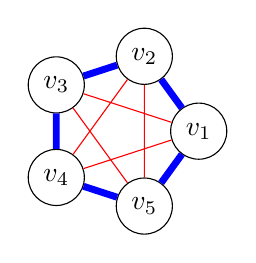
\begin{tikzpicture}[scale=1]
		\tikzstyle{every node}=[draw,shape=circle];
		\path (0:1cm)    node (v1) {$v_1$};
		\path (72:1cm)   node (v2) {$v_2$};
		\path (2*72:1cm) node (v3) {$v_3$};
		\path (3*72:1cm) node (v4) {$v_4$};
		\path (4*72:1cm) node (v5) {$v_5$};
		\draw[blue, line width = 2.5pt] (v1) -- (v2)
		(v2) -- (v3)
		(v3) -- (v4)
		(v4) -- (v5)
		(v5) -- (v1);
		\draw[red] 
		(v1) -- (v3)
		(v1) -- (v4)
		(v2) -- (v4)
		(v2) -- (v5)
		(v3) -- (v5);
		\end{tikzpicture}
	\end{center}
	\caption{Counter example for $K_5$}
	\label{fig:ramcounter}
\end{marginfigure}
The friendship statement is saying that $R(3) \leq 6$ and the counter-example shown in figure \ref{fig:ramcounter} shows that $R(3) >5$, so we obtain $R(3) = 6$. One might wonder if it is always possible to find monochromatic subgraphs of arbitrary size. Ramsey's theorem answers this question.
\begin{thm}[Ramsey]
	For any $k \in \N, R(k) < 4^k$, implying $R(k)$ is finite.
\end{thm}
Before giving a proof, we will look at the known bounds for some values of $k$. The obvious ones are $R(1) = 1$ and $R(2) = 2$ and more generally, $R(k) \geq k$. Next, $R(3) = 6$ which we have already seen and, although it takes a lot more work to prove, we know that $R(4) = 18$. Then, we hit a wall, the next numbers are not known but we do have some bounds. For example, we know that $42 < R(5) \leq 49$ and that $101 < R(6) \leq 165$. Let us digress a bit and quote Paul Erdos.

\begin{quote}
	"Suppose aliens invade the earth and threaten to obliterate it in a year's time unless human beings can find the [$R(5)$]. We could marshal the world's best minds and fastest computers, and within a year we could probably calculate the value. If the aliens demanded the [$R(6)$], however, we would have no choice but to launch a preemptive attack."
\end{quote}

While still postponing the proof of Ramsey's theorem, we look at a nice argument for the quadratic lower bound $R(k) > (k-1)^2$. To show this lower bound holds, we will construct a coloring on $E(K_{(k-1)^2})$ that does not have any monochromatic subgraph $K_k$. Divide the complete graph on $(k-1)^2$ vertices in $k-1$ groupings of $k-1$ vertices. Color the edges between the groupings in blue and the edges between the vertices of each grouping in red. Take any subgraph induced by $k$ vertices, all the vertices cannot be in the same grouping, so all the edges are not red. Also, all the vertices cannot be in different groupings, so all the edges are not blue.

\begin{defn}[General Ramsey number]
	We will use $R(k,\ell)$ to denote the minimal integer $n$ such that for any $2$-coloring of $E(K_n)$, we can either find a red $K_k$ or a blue $K_{\ell}$. Note that $R(k,k) = R(k)$. 
\end{defn}
We now show the finiteness of $R(k)$.
\begin{lem}
	\[R(k,\ell) \leq R(k-1, \ell) + R(k, \ell-1)\]
\end{lem}
\begin{proof}
	We will prove this by induction on $k+\ell$. For the base case, observe that for any $k$, $R(k,1) = R(1,k) = 1$ and $R(k,2) = R(2,k) = k$ since the subgraph induced by at most two vertices contains at most one edge, so it can only be monochromatic. If you cannot find two vertices connected by the color you want, then the whole graph must be of the other color so you found $K_k$ of the other color. You can now verify the inequality holds when $k+\ell \leq 5$.
	
	For the induction step, assume that it holds up until the sum is one less than $k+\ell \geq 6$ and fix some $2$-coloring of $E(K_n)$, where $n = R(k-1,\ell) + R(k, \ell -1)$ (we know these numbers are finite by the induction hypothesis). Pick an arbitrary vertex $v$ and observe that we have two cases. There is either at least $R(k-1,\ell)$ red neighbors of $v$ or at least $R(k,\ell-1)$ blue neighbors of $v$. For the first case, we use the induction hypothesis in the red neighbors to find a blue $K_{\ell}$ or a red $K_{k-1}$ from which we can create a red $K_k$ by adding $v$. For the second case, we use the induction hypothesis in the blue neighbors to find a red $K_k$ or a blue $K-{\ell-1}$ from which we can create a blue $K_{\ell}$ by adding $v$.
\end{proof}
A similar result can be used to obtain the upper bound stated in Ramsey's theorem.
\begin{lem}
	\[R(k,\ell) \leq \binom{k+\ell-2}{k-1}\]
\end{lem}
\begin{cor}
	$R(k) = R(k,k) < 4^k$
\end{cor}
\begin{proof}
	\[R(k,k) \leq \binom{2k-2}{k-1} < 2^{2k-2} < 4^k \]
	The second inequality is true because $2^{2k-2}$ is the number of subsets of a set of size $2k-2$ while $\binom{2k-2}{k-1}$ is the number of subsets of size $k-1$ of a set of size $2k-2$.
\end{proof}

\begin{proof}[Proof of lemma]
	The proof is really similar to the last lemma and uses induction. Again, we have two base cases : \begin{align*}
	R(1,k) = R(k,1) = 1 &\leq \binom{k+1-2}{k-1} = \binom{1+k-2}{k-1}\\
	R(2,k) = R(k, 2) = k &\leq \binom{k+2-2}{k-1} = \binom{2+k-2}{k-1}
	\end{align*}
	For the induction step, assume that the inequality holds up until the sum is one less than $k+\ell \geq 6$ and fix some coloring of $E(K_n)$ where $n = \binom{k+\ell-2}{k-1}$. Pick an arbitrary vertex $v$, we have two cases again. There is either at least $\binom{k+\ell-3}{k-2}$ red neighbors of $v$ or at least $\binom{k+\ell-3}{k-1}$ blue neighbors. Assume that none of these cases happen, then we obtain the following:
	\[ n \leq 1+\binom{k+\ell-3}{k-2}- 1 + \binom{k+\ell-3}{k-1}-1 = \binom{k+\ell-2}{k-1} -1 \]
	leading to a contradiction. The rest of the proof is the same as for the last lemma.
\end{proof}
Although this upper bound can be improved, we will instead focus on improving our lower bound with a more involved argument. We will argue to obtain a value as large as we can without actually constructing the graph (like we did for the last lower bound).

Fix some $k\geq 3$ and make the following definitions.\footnote{These definitions all depend on $n$ but we refrain from indicating in the notation to lighten the latter}
\begin{align*}
	\mathcal{C} &= \{ \mbox{all $2$-colorings of $E(K_n)$} \}\\
	\mathcal{C}_Y &= \{ c \in \mathcal{C} \mid \exists \mbox{ monochromatic } K_k \}\\
	\mathcal{C}_N &= \mathcal{C}\setminus \mathcal{C}_Y
\end{align*}
We are interested in the size of these collections. Observe that the size of $\mathcal{C}$ is $2^{\binom{n}{2}}$ and that our goal is to find an $n$ as large possible for which $|\mathcal{C}_N|$ or equivalently $|\mathcal{C}_Y| < |C|$. For a set $A \subseteq V(K_n)$ of size $k$ and define the following collections.
\begin{align*}
	R_A &= \{ c \in \mathcal{C} \mid \mbox{the complete subgraph induced by $A$ is red} \}\\
	B_A &= \{ c \in \mathcal{C} \mid \mbox{the complete subgraph induced by $A$ is blue} \}
\end{align*}
A simple combinatorics argument gives $|R_A| = |B_A| = 2^{\binom{n}{2} - \binom{k}{2}}$, also, we have 
\[ \mathcal{C}_Y = \bra{\bigcup_{\substack{A \subseteq V(K_n)\\|A| = k}} B_A} \cup \bra{\bigcup_{\substack{A \subseteq V(K_n)\\|A| = k}} R_A} \]
We will try to bound $|\mathcal{C}_Y|$ to see for what $n$ it is smaller than $|\mathcal{C}|$. We will use what is called the union bound which can be stated as follows for any set $X$ and $Y$.
\[|X \cup Y| = |X| +|Y| - |X \cap Y| \leq |X| + |Y| \]
We obtain the following derivation.
\begin{align*}
	|\mathcal{C}_Y| &\leq \left|\bigcup_{A}B_A\right| + \left|\bigcup_{A}R_A\right|&&\mbox{(union bound)}\\
	&= 2\left|\bigcup_{A}B_A\right|&&\mbox{(symmetry of colorings)}\\
	&\leq 2\sum_{A \in \binom{V}{k}} |B_A| &&\mbox{(union bound)}\\
	&= 2\binom{n}{k} \cdot 2^{\binom{n}{k}-\binom{k}{2}}&&\mbox{(counting)}\\
	&= n^k \cdot 2^{\binom{n}{k}-\binom{k}{2} + 1}&&\mbox{($\binom{n}{k} \leq n^k$)}\\
	&= 2^{\binom{n}{k}-\binom{k}{2} + 1 + k\log_2(n)}&&\mbox{(properties of exponent)}
\end{align*}
If we want to know when $|\mathcal{C}_Y| < |\mathcal{C}|$, we need to solve for $n$ in $2^{\binom{n}{k}-\binom{k}{2} + 1 + k\log_2(n)} < 2^{\binom{n}{2}}$. This is equivalent to the following.
\begin{align*}
	\binom{n}{2} &> \binom{n}{k}-\binom{k}{2} + 1 + k\log_2(n)\\
	\binom{k}{2} &> 1 + k\log_2(n)\\
	\frac{k^2-k}{2} &> 1 + k\log_2(n)\\
	k &> 2\log_2(n) + \frac{2}{k} + 1\\
\end{align*}
Choose $n=2^{\frac{k-2}{2}}$ to obtain $k > k-2+1+\frac{2}{k}$ which holds for $k \geq 3$. This is our lower bound for $R(k)$.
\begin{rem}
	Before further generalizing the Ramsey numbers, we want to point out that $R(k)$ can also be viewed as the minimal integer $n$ such that any graph on $n$ vertices contains either a complete subgraph on $k$ vertices or an empty one (equivalently, $\alpha(G) \geq k$).
\end{rem}
\begin{defn}[More general Ramsey number]
	We use $R_{\ell}(k)$ to denote the minimal integer $n$ such that for any $\ell$-coloring of $E(K_n)$, we can find a monochromatic subgraph induced by $k$ vertices. We can also use $R_{\ell}(k_1, \dots, k_{\ell})$ to denote the minimal integer $n$ such that for any $\ell$-coloring of $E(K_n)$, we can either find a $K_{k_1}$ of color $k_1$ or a $K_{k_2}$ of color $k_2$, etc...
\end{defn}
\begin{thm}
	For any $\ell$ and $k$, $R_{\ell}(k)$ is finite.
\end{thm}
\begin{proof}
	We prove it by induction, for $\ell=1,2$ the proof is already done. Assume that the theorem holds up to some $\ell$, we claim that
	\[R_{\ell+1}(k) = R_{\ell+1}(k,\stackrel{\ell+1}{\dots}, k) \leq R_{\ell}(k, \stackrel{\ell-1}{\dots},k,R_2(k,k))\]
	Take any complete graph of size bigger than the R.H.S. and any $(\ell+1)$-coloring $c$. Reduce this coloring to an $\ell$-coloring by combining the colors $\ell$ and $\ell+1$ together. If we can find a monochromatic $K_k$ of color in $\{1,\dots, \ell-1\}$, we are done because it will be also monochromatic with the coloring $c$. If we cannot find such coloring, then we must be able to find a monochromatic $K_{R_2(k)}$. If we look at this subgraph with the coloring $c$, it has only two colors so it must contain a monochromatic $K_k$ of color $\ell$ or $\ell+1$.
\end{proof}
We now use the Ramsey numbers in a number theoretic puzzle.
\begin{quest}
	Can you color the natural numbers\footnote{We are working with $\N^+$ since $0+0=0$ would always be a monochromatic solution} with red and blue such that there is no monochromatic solution to $x+y=z$ ?
\end{quest}
By a monochromatic solution, we mean that $c(x)=c(y)=c(z)$ and $x+y = z$. Let us start coloring and see what happens. By symmetry, we can arbitrary choose 1 to be red. Since $1+1=2$, 2 must be blue to have a valid coloring. Since $2+2=4$, 4 must be colored red and then $1+4=5$ means 5 must be blue. Then, 3 can be either red or blue. In the first case, $1+3=4$ is a monochromatic solution. In the second case, $2+3 = 5$ is a monochromatic solution.

In fact, it is possible to generalize this result to any numbers of colors.
\begin{thm}[Schur]
	For any $\ell \in \N$, $\N^+$ is not $\ell$-colorable such that $x+y=z$ has no monochromatic solution.
\end{thm}
\begin{proof}
	We will prove an equivalent statement : for any $\ell \in \N$, there exists an integer $n(\ell)$ such that any $\ell$-coloring of $\{1,\dots, n(\ell)\}$ has a monochromatic solution to that equation.
	
	We claim that $n(\ell) = R_{\ell}(3) -1$. Denote $c$ to be an arbitrary $\ell$-coloring of $\{1,\dots, n(\ell)\}$. Take the complete graph on the integers $\{1,\dots, R_{\ell}(3)\}$ and consider the following $\ell$-coloring $d$ of $E(K_{R_{\ell}(3)})$ : $\forall i< j, d(\{i,j\}) = c(j-i)$. Note that $1 \leq j-i \leq R_{\ell}(3)-1$ so this is well defined. By the definition of $R_{\ell}(3)$, there exists a monochromatic triangle in $d$. Namely, there exists integers $x<y<z$ such that $d(\{x,y\}) = d(\{y,z\}) = d(\{x,z\})$. However, by how we defined $d$, this is equivalent to $c(y-x) = c(z-y) = c(z-x)$. We get a monochromatic solution since $y-x + z-y = z-x$.
\end{proof}

\section{Connectivity of graphs}
This section will introduce the notion of connectivity. This part of graph theory arose during the war, when Russian were trying to figure out how to disconnect the railway network by destroying the least amount of connections. Another problematic was to find the maximal amount of resources could be sent through the same network. As it turns out these two problems lead to the same theory.

There are two ways to define connectivity in a graph, using the vertices or the edges. We will study those in parallel as the results will be similar but not always the same.

\begin{defn}[Vertex-disjoint paths]
	Let $G=(V,E)$ be a simple graph and $u \neq w \in V$. We will use $P_G(u,w)$ to denote the maximal size of a collection of internally vertex-disjoint paths from $u$ to $w$. By internally vertex-disjoint, we imply that all vertices except for $u$ and $w$ are in at most one path of the collection.
\end{defn}
Clearly, $P_G(u,w)$ is positive and $P_G(u,w) = 0$ if and only if $u \not\sim w$. Moreover, since paths cannot contain the same vertices and at most one path contains only 2 vertices, we have $P_G(u,w) \leq |V|-1$. We define the connectivity of $G$ as follows :
\[ \kappa(G) = \min_{u \neq w \in V}P_G(u,w) \]
One can remark that $\kappa(G) = 0$ if and only if $G$ is disconnected.

\begin{defn}[Edge-disjoint paths]
	Let $G=(V,E)$ be a multigraph and $u \neq w \in V$. We will use $P'_G(u,w)$ to denote the maximal size of a collection of edge-disjoint paths. By edge-disjoint, we imply that all edges are in at most one path of the collection.
\end{defn}
Once again, $P'_G(u,w)$ is positive and zero if and only if $u \not\sim w$. However, since we are working in a multigraph, it is impossible to give an upper bound. Indeed, the graph could have an arbitrary number of edges from $u$ to $w$ and $P'_G(u,w)$ would be at least this number. The new definition of connectivity we give is the following :
\[ \kappa'(G) = \min_{u \neq w \in V} P'_G(u,w) \]
\begin{exmps}
	\begin{itemize}
		\item For an empty graph on a single vertex, we have $\kappa(G) = \kappa'(G) = 1$.
		\item For a complete graph, we have $\kappa(K_n) = \kappa'(K_n) = n-1$.
		\item For a tree $T$, we have $\kappa(T) = \kappa'(T) = 1$ since all there are unique paths between any vertices.
		\item For a cycle, we have $\kappa(C_n) = \kappa'(C_n) = 2$ since you can only go from a vertex to another by following the cycle in one orientation or the other.
		\item These two values are not always the same. For a graph composed of two cliques\footnote{A clique is a synonym for a complete subgraph} of size $n_1$ and $n_2$ with 2 vertices in common, we have $\kappa(G) =2$ and $\kappa'(G) = \min(n_1-1, n_2-1)$.
	\end{itemize}
\end{exmps}
\begin{defn}[Vertex cut]
	A subset $C \subseteq V$ is a vertex cut if $G[V\setminus C]$ is disconnected. $\{v\}$ is a vertex cut if and only if $v$ is a cut vertex.
\end{defn}
For any vertex cut $C$, $\kappa(G) \leq |C|$ because if $G[V\setminus C]$ has two connected components $A$ and $B$, the vertices $u \in A$ and $w \in B$ have at most $|C|$ vertex disjoint paths between them, otherwise they would still be connected.
\begin{thm}[Menger]
	Let $G$ be a simple and not complete graph, then \[\kappa(G) = \min_{C \mbox{ vertex cut}} |C|\]
\end{thm}
\marginnote{In the literature, you might find this to be the definition of connectivity}
\begin{defn}[Edge cut]
	A subset $F \subseteq E$ is an edge cut if $G' = (V, E\setminus F)$ is disconnected. $\{e\}$ is an edge cut if and only if $e$ is a cut edge.
\end{defn}
For any edge cut $F$, $\kappa'(G) \leq |F|$ because if $G'$ has two connected components $A$ and $B$, the vertices $u \in A$ and $v\in B$ have at most $|F|$ edge disjoint paths between them, otherwise they would still be connected.
\begin{thm}[Ford-Fulkerson]
	Let $G$ be a multigraph, then \[\kappa'(G) = \min_{F \mbox{ edge cut}} |F|\]
\end{thm}

In order to prove these theorems, we will use a prove two lemmas, one can view these as the "local" versions of the theorems.
\begin{defn}
	Let $G = (V,E)$ be a graph and $u \neq w \in V$ such that $\{u,w\} \notin E$. We will use $c_G(u,w)$ to denote the minimum size of a vertex cut $C$ not containing $u$ nor $w$ such that $C$ disconnects $u$ and $w$.
\end{defn}
\begin{lem}
	Let $G=(V,E)$ be a simple graph. For any $u \neq w \in V$ such that $\{u,w\} \notin E$, we have $c_G(u,w) = P_G(u,w)$.
\end{lem}
\begin{proof}
	We will use induction on $|E|$, the base case $|E| = 0$ is trivial. For the induction step, assume for all graphs with less edges than $G$ and let $u\neq w \in V$ be two non-adjacent vertices. Also, denote $k = c_G(u,w)$. It is clear that $P_G(u,w) \leq k$ because if you remove $k$ vertices in those disjoint paths, $u$ and $w$ must become disconnected. The other inequality is less trivial and involves two cases.
	\begin{marginfigure}
	\centering
	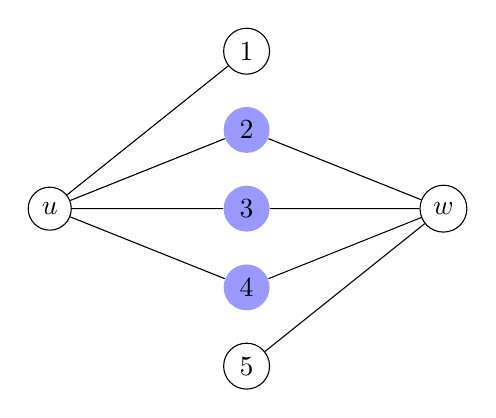
\begin{tikzpicture}[neigh_node/.style={circle,fill=blue!40,minimum size=1em,inner sep=3pt}, main_node/.style={circle,draw,minimum size=1em,inner sep=3pt}]
	
	\node[main_node] (1) at (0,0) {$u$};
	\node[main_node] (2) at (5, 0)  {$w$};

	\node[main_node] (a) at (2.5, 2) {$1$};
	\node[neigh_node] (b) at (2.5, 1) {$2$};
	\node[neigh_node] (c) at (2.5, 0) {$3$};
	\node[neigh_node] (d) at (2.5, -1) {$4$};
	\node[main_node] (e) at (2.5, -2) {$5$};
	
	\draw (1) -- (a)
(1) -- (b)
(1) -- (c)
(1) -- (d)

(2) -- (b)
(2) -- (c)
(2) -- (d)
(2) -- (e);
	\end{tikzpicture}
	\caption{This is an example of a graph for the first case, the highlighted nodes are in the intersection of the neighborhoods and form the only vertex cut separating $u$ and $w$}
\end{marginfigure}
	Suppose that every edge in $E$ has an endpoint in $\{u,w\}$. The minimal vertex cut is the only vertex cut separating $u$ and $w$, namely, $C= N_G(u) \cap N_G(w)$. This is true because removing these vertices will disconnect $u$ and $w$ and any other subset of $V$ will either contain $u$ or $w$ or it will not contain some vertex in $C$, leaving $u$ and $w$ connected via that vertex. Also, we clearly have $P_G(u,w) = |C| = k = c_G(u,w)$ and we are done.
	
	In the second case, there exists some edge $f = \{a,b\}$ where $f \cap \{u,w\} = \emptyset$. Define a new graph $H = G-f$ and observe that $P_H(u,w) \leq P_G(u,w)$ since all the paths in $H$ are paths in $G$. Also, we have $c_G(u,w) \leq c_H(u,w) + 1$ since if $C$ is a cut disconnecting $u$ and $w$ in $H$, then $C\cup \{a\}$ must disconnect $u$ and $w$ as well. We can rewrite this inequality as $c_H(u,w) \geq k-1$ and our induction hypothesis gives $P_H(u,w) = c_H(u,w) \geq k-1$ because $H$ has less edges than $G$. If both of these are actually equal to $k$, then we must have $P_G(u,w) = k$ and we are done. Assume otherwise and denote $C = \{v_1, \dots, v_{k-1}\}$ be a vertex cut disconnecting $u$ and $w$.
	
	Going back to the graph $G$, we know that $C$ does not disconnect $u$ and $w$ because $|C| < c_G(u,w) = k$. This implies that there is a path from $u$ to $w$ passing through the edge $f$. Without loss of generality, say that $u,a \in U$ and $w,b \in W$ where $U$ and $W$ are components of $H-C$. Define the following graphs :
	\begin{align*}
		G_u &= \bra{ (V \setminus U)\cup \{\bar{u}\}, E_u)} \\&\mbox{ where } E_u = \{ e \in E \mid e \cap U = \emptyset \} \cup \left\{\{\bar{u},y\} \mid x \in U, \{x,y\} \in E \right\}\\
		G_w &= \bra{ (V \setminus W)\cup \{\bar{w}\}, E_w)} \\&\mbox{ where } E_w = \{ e \in E \mid e \cap W = \emptyset \} \cup \left\{\{\bar{w},y\} \mid x \in W, \{x,y\} \in E \right\}
	\end{align*}
	 Note that any vertex cut in $G_u$ that separates $\bar{u}$ and $w$ will separate $u$ and $w$ in $G$ as well. Hence, $c_{G_u}(u,w) \geq k$. On the other hand, the vertex cut $\overline{C} = C \cup \{b\}$ separates $\bar{u}$ and $w$ in $G_u$ so $c_{G_u}(\bar{u}, w) =k$.
	 
	 We can use the induction hypothesis on $G_u$ because all edges coming out $U$ are represented by at most one edge per vertex not in $U$ and at least one edge inside $U$ is removed because $u, a\in U$. Therefore, we have $k$ internally disjoint paths from $\bar{u}$ to $w$, denoted $P_1, \dots, P_k$. With a symmetric argument for $G_w$, we obtain a collection $Q_1, \dots, Q_k$ of internally disjoint paths from $\bar{w}$ to $u$. Each paths in each collection must go through $\overline{C}$ and they are disjoint, so they pass by exactly one vertex in $\overline{C}$. Without loss of generality, say that $P_i$ and $Q_i$ pass through $v_i$ for $i \in \{1,\dots, k-1\}$ and say $P_k$ and $Q_k$ pass through $a$ and $b$ respectively.
	 
	 We will construct $k$ internally disjoint paths in $G$. For $i \in \{1,\dots, k-1\}$, the path starting at $u$, following $Q_i$ until $v_i$ and then following $P_i$ until $w$ will be internally disjoint from the path with the same construction and $j \neq i$. This gives $k-1$ paths. The last one starts at $u$ and follows $Q_k$ until $a$ goes to $b$ with the edge $f$ and follows $P_k$ until $w$.
\end{proof}
We use this lemma to prove Menger's theorem.
\begin{proof}[Proof of Menger]
	Let $G = (V,E)$ be simple and not complete, so there exists some vertices which are not adjacent. Pick $u \neq w \in V$ such that $P_G(u,w)$ is minimal and denote $\kappa(G) = k$. If $u$ and $w$ are not adjacent, then using the lemma, $c_G(u,w) = P_G(u,w) = k$.
	
	Suppose that $u$ and $w$ are adjacent and consider the graph $H= (V, E\setminus \{u,w\})$. We clearly have $P_H(u,w) = P_G(u,w) -1 = k-1$ and from the lemma, we obtain $c_H(u,w) = k-1$. Let $C$ be a vertex cut of size $k-1$ separating $u$ and $w$. Assume towards a contradiction that $C = V \setminus \{u,w\}$, then $|C| = |V|-2$ implying that $k=|V|-1$ and we have seen that this implies $G$ is complete, leading to a contradiction.
	
	We can now pick some vertex $x \in V(H) \setminus C$ with $x \neq u$ and $x \neq w$. Without loss of generality, in $H-C$, $x$ is not connected to $w$, implying that $C \cup \{u\}$ separates $x$ and $w$. We get $c_G(x,w) \leq k$, so we found a vertex cut of size $k$.
\end{proof}
\begin{defn}
	Let $G = (V,E)$ be a graph and $u \neq w \in V$. We will use $c'_G(u,w)$ to denote the minimum size of an edge cut $F$ such that $F$ disconnects $u$ and $w$.
\end{defn}
\begin{lem}
	Let $G=(V,E)$ be a multigraph. For any $u \neq w \in V$, we have $c'_G(u,w) = P'_G(u,w)$.
\end{lem}
We can view this lemma in a different way which somewhat links this to the next section.
\begin{defn}[Boundary]
	Let $X \subseteq V(G)$, we define the boundary of $X$ (denote it $\partial(X)$) as the set of edges touching exactly one vertex of $X$, namely, $\partial(X) = \{e \in E \mid |e \cap X| = 1\}$.
\end{defn}
\begin{rem}
	Observe that \[c'_G(u,w) = \min_{\{u\} \subseteq X \subseteq V \setminus \{w\}} |\partial_G(X)| =  \]
\end{rem}

In order to prove this result and Ford-Fulkerson's theorem, we will develop a more general theory about networks and flows.

\section{Networks}
As usual when starting a new section, we will start with a series of definitions and observations to get familiar with the objects we will work with.
\begin{defn}[Digraph]
	A digraph $D$ is a tuple $(V,E)$ where $E \subseteq V \times V$. The edges are now ordered pairs and contain information about the orientation of the edge. It is different from an oriented graph since it could have two edges that go from one vertex to another and back, namely, for $v,w \in V$, $(v,w), (w,v) \in E$.
\end{defn}
\begin{defn}[Directed path]
	A directed path in $D$ is a path $P = \{v_0,e_1,v_1, \dots, e_k, v_k\}$ such that $e_i = (v_{i-1},v_i)$. $P$ goes from $v_0$ to $v_k$ and not the opposite.
\end{defn}
\begin{defn}[Oriented boundaries]
	Let $X \subseteq V$, we define the oriented boundaries of $X$:
	\begin{align*}
		\partial^+(X) &= \{ (u,w) \in E \mid u \in X, w \notin X \} = \mbox{outgoing edges}\\
		\partial^-(X) &= \{ (u,w) \in E \mid u \notin X, w \in X \} = \mbox{incoming edges}
	\end{align*}
\end{defn}
\begin{lem}
	Let $D = (V,E)$ be a digraph and $s \neq t \in V$, then either there exists a directed path from $s$ to $t$ or there exists a subset $X \subseteq V$ with $\{s\} \subseteq X \subseteq V \setminus\{t\}$ such that $\partial^+(X) = \emptyset$.
\end{lem}
\begin{proof}
	Let $X = \{x \in V \mid \exists \mbox{ directed path from } s \mbox{ to } x \}$. Clearly $\partial^+(X) = \emptyset$ as if it were not empty, there would be a directed path from $s$ to the head of an edge in the boundary, so the head must be in $X$ which is a contradiction. Also, $s \in X$ by the empty path. Now, either $t \in X$ and there exists a directed path from $s$ to $t$ or $t \notin X$ and $X$ is the desired subset.  
\end{proof}
\begin{defn}[Flow]
	Let $D= (V,E)$ be a digraph and $s\neq t \in V$. A map $\phi : E \rightarrow \R^+_0$ is an $s,t$-flow if $\forall x \in V \setminus\{s,t\}$, the following holds\footnote{This is often called Kirchoff's law, you might recognize it from a course in electromagnetism}:
	\[ \sum_{e \in \partial^+(x)}\phi(e) = \sum_{e \in \partial^-(x)}\phi(e) \]
	We define the value of an $s,t$-flow as follows:
	\[ \val(\phi) = \sum_{e \in \partial^+(s)}\phi(e) - \sum_{e \in \partial^-(s)}\phi(e) = \sum_{e \in \partial^-(t)}\phi(e) - \sum_{e \in \partial^+(t)}\phi(e)\]
\end{defn}
\begin{lem}
	Let $D=(V,E)$ be a digraph, $s\neq t$ be vertices and $\phi$ be an $s,t$-flow of value $k$, then $\forall \{s\} \subseteq X \subseteq V\setminus\{t\}$, we have 
	\[ \sum_{e \in \partial^+(X)}\phi(e) - \sum_{e \in \partial^-(X)}\phi(e) = k \]
\end{lem}
\begin{proof}
	Define the following subset of edges:
	\begin{align*}
		E_0 &= \{e \in E \mid |e \cap X| = 0 \}\\
		E_1 &= \{e \in E \mid |e \cap X| = 2 \}\\
		E_H &= \{(u,w) \in E \mid u \notin X, w \in X\}\\
		E_T &= \{(u,w) \in E \mid w \notin X, u \in X\}
	\end{align*}
	It is obvious that $E = E_0 \cup E_1 \cup E_H \cup E_T$ and that all this sets are disjoint. Also, note that $E_H = \partial^-(X)$ and $E_T = \partial^+(X)$.
	\begin{align*}
		k &= \sum_{e \in \partial^+(s)} \phi(e) - \sum_{e \in \partial^-(s)}\phi(e)\\
		&=\sum_{x \in X} \bra{\sum_{e \in \partial^+(x)} \phi(e) - \sum_{e \in \partial^-(x)}\phi(e)}\\
		&= \sum_{e \in E_0} 0 + \sum_{e \in E_1}0+ \sum_{e \in E_H} -\phi(e) + \sum_{e \in E_T} \phi(e)\\
		&= \sum_{e \in \partial^+(X)}\phi(e) - \sum_{e \in \partial^-(X)}\phi(e)
	\end{align*}
\end{proof}
\begin{defn}[Capacity function]
	Let $D= (V,E)$ be a digraph, a capacity function is a map $c : E\rightarrow \R^+_0$.
\end{defn}
\begin{defn}[Network]
	A network is a 5-tuple $(V,E,s,t,c)$ where $(V,E)$ is a digraph, $s \neq t \in V$ are called the source and target(or sink) of the network and $c$ is a capacity function.
\end{defn}
\begin{defn}[$c$-admissibility]
	An $s,t$-flow is $c$-admissible if $\forall e \in E, \phi(e) \leq c(e)$.
\end{defn}
\begin{rem}
	Although all of the following theory will work when the range of $\phi$ is the positive real numbers, there is some theory about the maximum of functions in multidimensional spaces that needs to be used and we do not want to mention it in this class. Therefore, we will assume that $\phi$ is an integral function.
\end{rem}
\begin{lem}
	Let $D=(V,E)$ be a digraph, $s\neq t$ be vertices and $\phi$ be an integral $s,t$-flow of value $k$, then there exists a collection of paths $\{P_1, \dots, P_k\}$ all going from $s$ to $t$ such that every edge $e \in E$ belongs to at most $\phi(e)$ paths. 
\end{lem}
\begin{proof}
	We prove it by induction on $k$. When $k = 0$, the property is vacuously true.
	
	Suppose the property holds for $k-1$, with $k\geq 1$. Define $D' = (V, \{e \in E, \phi(e) > 0\})$. If there is no directed path from $s$ to $t$ in $D'$, by lemma 135, there exists a subset $\{s\} \subseteq X \subseteq V \setminus \{t\}$ such that $\partial^+(X) = \emptyset$. However, by lemma 137 and the fact that $\phi$ is positive, we get that $k<0$ which contradicts our beginning assumption.
	
	Let $P_k$ be a directed path form $s$ to $t$ in $D'$ and define the map $\psi : E \rightarrow \N_0$ as follows:
	\[ \psi(e) = \begin{cases}\phi(e) &e \notin P_k\\ \phi(e) -1 & e \in P_k\end{cases} \]
	Kirchoff's law still holds for every internal vertex in the path since we remove 1 from an outgoing edge and 1 from an incoming edge. Hence, this map is an $s,t$-flow in $D$. Moreover, $\val(\psi) = k-1$ since we remove 1 from exactly one outgoing edge of $s$. We can now use the induction hypothesis to find paths $P_1, \dots, P_{k-1}$ such that every edge $e$ in $D$ is in at most $k-1$ paths. Adding the last path $P_k$ still maintains the desired property.  
\end{proof}
\begin{defn}[Augmenting path]
	An undirected path $P = \{v_0,e_1,\dots, e_{\ell},v_{\ell}\}$ from $s$ to $t$ in a network $(V,E,s,t,c)$ is called augmenting for an $s,t$-flow $\phi$ if $\forall i \in \{1,\dots, \ell\}$, $e_i = (v_i,v_{i+1}) \implies \phi(e) \leq c(e) - 1$ and $e_i = (v_{i+1}, v_i) \implies \phi(e) \geq 1$.
\end{defn}
\begin{lem}
	Let $(V,E,s,t,c)$ be a network, $\phi$ be an integral $c$-admissible $s,t$-flow and $P$ be an augmenting path for $\phi$. Then there exists a $c$-admissible $s,t$-flow $\psi$ with $\val(\psi) \geq \val(\phi) + 1$.
\end{lem}
\begin{proof}
	Define the following map :
	\[ \psi(e) = \begin{cases} \phi(e)+1 &\mbox{if $P$ uses $e$ in the forward direction}\\
	\phi(e)-1 &\mbox{if $P$ uses $e$ in the backward direction}\\
	\phi(e) &\mbox{otherwise}\end{cases} \]
	Observe that $\forall e\in E, 0\leq \psi(e) \leq c(e)$ by the definition of an augmenting path and the map $\psi$. Let $x \in V \setminus \{s,t\}$ inside the path $P$. Say that $x$ appears in the path in the following sequence $vexfw$ where $v,w \in V$ and $e,f \in E$. We have four cases.
	\begin{itemize}
		\item $e = (v,x)$ and $f=(x,w)$ yields $\psi(e) = \phi(e) + 1$ and $\psi(f) = \phi(f) +1$
		\item $e = (v,x)$ and $f=(w,x)$ yields $\psi(e) = \phi(e) + 1$ and $\psi(f) = \phi(f) - 1$
		\item $e = (x,v)$ and $f=(x,w)$ yields $\psi(e) = \phi(e) - 1$ and $\psi(f) = \phi(f) +1$
		\item $e = (x,v)$ and $f=(w,x)$ yields $\psi(e) = \phi(e) - 1$ and $\psi(f) = \phi(f) - 1$
	\end{itemize}
	All these four cases maintain Kirchoff's property for $x$ showing that $\psi$ is an $s,t$-flow. Moreover, $\val(\psi) = \val(\phi)+1$ since we either add 1 to the flow of an outgoing edge or we remove 1 from the flow of an incoming edge. This finishes the proof of the lemma.
\end{proof}
We are now going to show the main result of this section. This is the network version of the Ford-Fulkerson theorem we have introduced in the last section.
\begin{defn}[Capacity of a set]
	Let $(V,E,s,t,c)$ be a network and $\{s\} \subseteq X \subseteq V\setminus\{t\}$. The capacity of the set is denoted $\capac(X)$ and defined \[\capac(X) = \sum_{e \in \partial^+(X)} c(e)\]
\end{defn}
\begin{thm}[Ford-Fulkerson]
	Let $(V,E,s,t,c)$ be a network and $\Phi$ be the set of all $c$-admissible $s,t$-flows, then, we have the following:
	\[ \max_{\phi \in \Phi} \val(\phi) = \min_{\{s\} \subseteq X \subseteq V \setminus \{t\}} \capac(X) \]
\end{thm}
\begin{proof}
	For the $\leq$ side, let $\{s\} \subseteq X \subseteq V \setminus \{t\}$ be an $s,t$-cut of minimum capacity $k$. Clearly, any flow needs to pass through $X$ so it cannot have a value more than $k$.
			
	For the $\geq$ side, let $\phi$ be an $s,t$-flow of maximum value $k$. Let $X = \{x \in V \mid \exists \phi\mbox{-augmenting path from } s \mbox{ to } x\}$. By Lemma 144, we know that there cannot be an augmenting path for $\phi$ so $t \notin X$. Also, $s \in X$ by the empty path. Moreover, we have that $\forall e \in \partial^+(X), \phi(e) = c(e)$ and $\forall e \in \partial^-(X), \phi(e) = 0$, otherwise we would $e$ would extend an augmenting path outside $X$. Therefore, we use Lemma 137 to obtain
	\[ k = \sum_{e \in \partial^+(X)} c(e) = \capac(X) \]
	This shows that $k \geq \min_{\{v\} \subseteq X \subseteq V \setminus \{t\}} \capac(X)$.
\end{proof}

In the next section, we go back to undirected graphs.
\section{Proper Vertex Coloring}
Recall that a graph $G$ is called bipartite if $V(G) = R \cup B$ such that $G[R]$ and $G[B]$ are empty. In this section, we try to generalize this notion.
\begin{defn}[Proper vertex coloring]
	Let $G = (V,E)$ be a simple graph. A proper $k$-vertex coloring of $G$ is a map $c: V \rightarrow \{1,\dots, k\}$ such that $\forall v \neq w \in V, c(v) \neq c(w)$, namely there is no monochromatic edge. The chromatic number of $G$, denoted $\chi(G)$, is the minimum $k$ such that there exists a proper $k$-vertex coloring of $G$.
\end{defn}
\begin{exmps}
	\begin{itemize}\item[]
		\item If $B$ is a bipartite graph with at least one edge, then $\chi(B) = 2$.
		\item If $G$ has no edges, $\chi(G) = 1$.
		\item For an even cycle, we have $\chi(C_{2\ell}) = 2$. For an odd cycle, we have $\chi(C_{2\ell + 1}) = 3$
		\item $\chi(K_n) = n$
	\end{itemize}
\end{exmps}
\begin{prop}
	Let $G$ be a simple graph, recall that $\alpha(G)$ is the size of the largest independent set. We have $\chi(G) \geq \frac{|V(G)|}{\alpha(G)}$.
\end{prop}
\begin{proof}
	Let $c$ be a proper vertex $k$-coloring and denote $V = X_1 \cup \cdots \cup X_k$ where $X_i = \{x \in V \mid c(x) = i\}$. Clearly, each set $X_i$ is independent, so we have the following:
	\[ |V| = \sum_{i=1}^k |X_i| \leq \alpha(G) \cdot k \leq \alpha(G) \cdot \chi(G) \]
	The inequality follows.
\end{proof}
\begin{rem}
	If $H \subseteq G$ and $\chi(H) \geq k$, then $\chi(G) \geq k$.
\end{rem}
We might ask what makes the chromatic number of $G$ bigger. One might notice that large cliques imply a large chromatic number and wonder if the converse is true. In fact, it is not and the following theorem shows that in a really strong sense.
\begin{defn}[Clique number]
	For a graph $G$, we define the clique number of $G$, and denote $\omega(G)$, to be the maximum number $\ell$ such that $K_{\ell} \subseteq G$.
\end{defn}
It is easy to see that $\chi(G) \geq \omega(G)$, but that bound is not that tight since we can construct a triangle free graph with chromatic number $k$, for any $k$.
\begin{thm}
	For any $k \in \N$, there exists a graph $G_k$ simple graph with no triangles and $\chi(G_k) > k$.
\end{thm}
\begin{proof}
	Fix some $k \in \N$. Let $n = R_k(3)$ and $N = \binom{n}{2}$, it is the number of edges in $K_n$. Let $G_k = (V,E)$ where $V$ contains all the edges $K_n$ and $E$ contains all the edges $\{\{a,b\}, \{c,d\}\}$ with $a<b = c<d$. We first claim that $G_k$ is triangle-free. Suppose that some vertices $\{a,b\}$, $\{c,d\}$ and $\{e,f\}$ form a triangle. Without loss of generality, we have the following two options :
	\begin{align*}
	a < b = c < d = e < f = a\\
	a < b = c < d = e < f = b
	\end{align*}
	Both lead to a contradiction. The second claim is that $\chi(G_k) > k$, i.e: for any map $c : V \rightarrow \{1,\dots, n\}$, there exists $e \in E$ such that both ends of $e$ have the same color in $c$. Fix some $c$ and observe that it is already a coloring of the edges of $K_n$ because these edges are the vertices of $G_k$. By the definition of the Ramsey number $R_k(3)$, there exists a monochromatic triangle in $K_n$. Namely, there exists $x < y< z \in \{1,\dots, n\}$ such that $c(\{x,y\}) = c(\{y,z\})$. This shows that $c$ is not a proper coloring.
\end{proof}
\begin{thm}
	Let $G = (V,E)$ be a graph without triangles with $n = |V|$, then $\chi(G) \leq \sqrt{2n}$.
\end{thm}
\begin{proof}
	Without loss of generality, we assume that $G$ is connected and prove it by induction on $n$. For the base case $n=1$, we have $\chi(G) = 1 \leq \sqrt{2}$. Suppose it holds for values smaller than $n$, with $n > 1$, we consider two cases.
	
	If $\forall v \in V, \deg(v) \leq \lfloor \sqrt{2n} \rfloor =: k$, by Brooks' theorem, we have $\chi(G) \leq \lfloor \sqrt{2n} \rfloor$ unless $G = K_n$ or $G = C_n$ when $n$ is odd. For the complete graph, $n$ must be 2 since otherwise $G$ would not be triangle-free. If $G = K_2$, we have $\chi(K_2) =2 \leq \sqrt{4}$. For the odd cycle, $n$ must be at least 5 since $C_3$ has a triangle. If $G = C_n$ with $n \geq 5$ an odd integer, we have $\chi(G) = 3 \leq \sqrt{2n}$.
	
	If $\exists v \in V$ with $\deg(v) \geq k+1 \geq \lceil \sqrt{2n} \rceil$. We have that $N(v)$ is an independent set of size at least $k+1$. Denote $G' = G-N(v)$. By induction, $\chi(G') \leq \sqrt{2(n-\lceil \sqrt{2n} \rceil)}$, implying that $\chi(G) \leq \sqrt{2(n-\lceil \sqrt{2n} \rceil)} +1$. Since you would need just one color for $N(v)$. Now, our aim is to show $\sqrt{2(n-\lceil \sqrt{2n} \rceil)} +1 \leq \sqrt{2n}$. We have the following equivalences.
	\begin{align*}
	\sqrt{2(n-\lceil \sqrt{2n} \rceil)} +1 &\leq \sqrt{2n}\\
	\sqrt{2(n-\sqrt{2n})} &\leq \sqrt{2n}-1\\
	2n-2\sqrt{2n} &\leq 2n-2\sqrt{2n} +1 &&\mbox{(by squaring both sides)}
	\end{align*}
\end{proof}
\begin{defn}[Maximum degree]
	We will denote $\Delta(G)$ to be the maximum degree of a vertex in $G$.
\end{defn}
Another easy observation is that $\chi(g) \leq \Delta(G) + 1$, but we can make this bound tighter with the following theorem.
\begin{thm}[Brooks]
	Let $G$ be a connected loopless multigraph that is not complete nor an odd cycle, then $\chi(G) \leq \Delta(G)$.
\end{thm}
\begin{proof}
	Pretty long proof that we might not do in class.
\end{proof}
\begin{defn}[$d$-degeneracy]
	A graph $G$ is called $d$-degenerate, if $\exists v \in \deg(v) \leq d$ and $G-v$ is also degenerate. Equivalently, every subgraph of $G$ has a vertex of degree less or equal to $d$.
\end{defn}
\begin{prop}
	If $G$ is $d$-degenerate, then $\chi(G) \leq d+1$.
\end{prop}
\begin{proof}
	We use induction on $n = |V|$. If $n = 1$, this is trivial. Now, assume it holds up to $n-1$. Then take a vertex $v \in V, \deg(v) \leq d$, by induction, you can color $G-v$ with $d+1$ colors since $G-v$ is also $d$-degenerate. Now, since $v$ has at most $d$ neighbors, there is one color that was not used in $N(v)$. Thus, we can finish the coloring of $G$ with that color.
\end{proof}
\begin{defn}
	A proper $k$-edge-coloring of a loopless multigraph $G = (V,E)$ is a map $c: E \rightarrow \{1, \dots, k\}$ such that $\forall e,f \in E, c(e) \neq c(f)$. Namely, we can decompose $E = E_1 \cup \cdots E_k$ where each $E_i$ is a matching. $\chi'(G)$ is the minimum $k$ such that there exists a $k$-edge coloring for $G$.
\end{defn}
\begin{exmps}
	\begin{itemize}\item[]
		\item $\chi'(C_{2\ell}) = 2$
		\item $\chi'(C_{2\ell+1}) = 3$
		\item $\chi'(G) \geq \max_{v \in V(G)} \deg(v)$
	\end{itemize}
\end{exmps}
\begin{thm}[Vizing]
If $G$ is a simple graph, then $\chi'(G) \leq \Delta(G)+1$. If $G$ is not simple, then denote $\mu(G)$ to be the maximum multiplicity of an edge in $G$, we have $\chi'(G) \leq \Delta(G)+\mu(G)$.
\end{thm}
\begin{proof}
	Later...
\end{proof}
\begin{thm}[Konig's line coloring]
	If $G = (V,E)$ is a bipartite graph, then $\chi'(G) = \Delta(G)$.
\end{thm}
\begin{proof}
	We show this by induction on $n = |E|$. When $|E| = 1$, it is obvious that $\chi'(G) = 1 = \Delta(G)$. Assume this holds up to $n-1$ and we have a bipartite graph $G$ with $|E| = n$. Pick some edge $e = \{u,w\} \in E$ and define $G' = G - e$. Clearly, $G'$ is bipartite and $\max_{v \in V(G')}\deg_{G'}(v) \leq \Delta(G)$. Hence, by our induction hypothesis, there exists a proper edge coloring of $G'$ using $\Delta(G)$ colors. Also, note that $\deg_{G'}(u), \deg_{G'}(w) \leq \Delta(G)-1$, namely, there exists colors $\alpha_u$ and $\alpha_w$ such that no edge of those colors are incident to $u$ and $w$ respectively. If $\alpha_u = \alpha_w$, extend the coloring of $G'$ to a coloring of $G$ by coloring $e$ with $\alpha_u$ and we are done.
	
	Suppose that $\alpha_u \neq \alpha_w$. Consider the subgraph of $G'$ with all the edges colored with $\alpha_u$ or $\alpha_w$ and call it $H$. We know that this graph is composed of cycles and paths and that $\deg_H(u) = \deg_H(w) = 1$. Therefore, $u$ and $w$ can only be the ends of paths in $H$. We have two cases. 
	
	If $u$ and $w$ are not in the same connected components, then, on the path of $u$, change all the edges of color $\alpha_u$ to $\alpha_w$ and vice-versa. Now, no edge of color $\alpha_w$ is incident to $u$ and we can color $e$ with $\alpha_w$ to get a proper edge coloring of $G$. If $u$ and $w$ are on the same path $P$, they are the ends of that path. $P$ must be of even length because the edges must alternate color and the two end edges are of different colors. However, this implies that $P+e$ is an odd cycle contradicting the fact that $G$ is bipartite.
\end{proof}
\begin{thm}[Shannon]
	If $G$ is a loopless multigraph, $\chi'(G) \leq 3 \lceil \frac{\Delta(G)}{2} \rceil$.
\end{thm}
\begin{proof}
	Let $k = \lceil\frac{\Delta(G)}{2} \rceil$, there exists a graph $H \supseteq G$, that is $2k$-regular\footnote{Its construction is easy, create a copy G and connect parallel edges from vertices $v$ to their copy until they have degree $2k$}. $H$ splits into $k$ $2$-factors. We can color each of these with $3$ colors, so we can color $H$ (hence $G$) with $3k = 3\lceil\frac{\Delta(G)}{2} \rceil$ colors.
\end{proof}

\section{Structural graph theory}
This section will mostly review properties of planar graphs. There will be parts where we do not use lots of formalism since introducing it requires topology notions that are out of the scope of this course.
\begin{defn}[Planar graph]
	A graph $G$ is planar if it has a drawing in the plane $\R^2$ such the edges do not intersect themselves or other edges except at the vertices (which are points on the plane).
\end{defn}
\begin{exmps}
	\begin{itemize}\item[]
		\item Trees are planar graphs. Pick a root arbitrarily, draw it with its neighbors such that this part of the graph is planar. Now, zoom in on each neighbor, considering it as the root of the subtree it is the ancestor to. Draw the subtrees recursively.
		\item Cycles are planar graphs. Draw a circle and put as many points on it as there are vertices in the graph.
		\item Empty graphs are planar. Just draw the vertices on different points of the plane.
		\item What about complete graphs. We give planar drawings for $K_2$, $K_3$ and $K_4$, but we will see that $K_5$ is not planar.
		%***********DRAWINGS*****************
	\end{itemize}
\end{exmps}
That last example raises the following question.
\begin{quest}
	How can we show that a graph is not planar ?
\end{quest}
We quickly see that proofs by exhaustion are not possible here. Indeed, although graphs are finite, their drawing is on $\R^2$, so there is a continuum of possibilities to draw it. Here is a more formal definition of a drawing.
\begin{defn}[Drawing]
	Let $G=(V,E)$ be a graph. A drawing or plane graph $D$ for $G$ in $\R^2$ is the following list of functions. First, there is an injective (so that no two vertices touch) map $f_{\sigma} : V \rightarrow \R^2$ that determines the position of each vertices. Then, for every edge $e = \{u,w\} \in E$, there is an injective (so that it is non self-intersecting) continuous map $f_e : [0,1] \rightarrow \R^2$ such that $f_e(0) = f_{\sigma}(u)$, $f_e(1) = f_{\sigma}(w)$ and $f_e((0,1)) \cap \im(f_{\sigma}) = \emptyset$. In other words, $f_e$ defines a non self-intersecting curve that starts at the position of $u$ and ends at the position of $w$ and does not cross the position of any other vertex. We further require that for any two edge $e = e'$, $\im(f_e) \cap \im(f_{e'}) \subseteq \im(f_{\sigma})$. This condition along with the definitions of $f_e$ and $f_{e'}$ states that the curves may only cross at a common endpoint of both edges.
\end{defn}
Seeing how long and involved this definition is, we see why we introduced this section by saying we were not going to do lots of formalism. This definition is too heavy and we will not use it in developing the theory for planar graphs. However, we will use the next theorem without proof since it helps us defining a region, which will be key in the following results.
\begin{thm}[Jordan's curve theorem]
	Any continuous non self-intersecting loop in the plane divides the plane in exactly two regions.
\end{thm}
\begin{rem}
	If $G$ is a planar graph and $H$ is a subgraph, then $H$ is planar. Pick a drawing for $G$ and remove all the vertices and edges not in $H$, the result is a drawing for $H$. The converse does not hold as we have seen that $K_5$ is not planar but $K_4$ is a planar subgraph of $K_5$. 
\end{rem}
As we have said before, the number of representations is too big for us to study, therefore, we will instead study properties of drawings and especially invariants.
\begin{defn}[Region]
	Let $G$ be a planar graph and $D$ its drawing in $\R^2$. A region\footnote{This is sometimes called a face} in $(G,D)$ is a maximal subset of the plane $S \subseteq \R^2$ such that $S$ is connected in the topological sense\footnote{Out of the scope for this class but you should follow your intuition on what defines a connected region} and $S$ is disjoint from all the vertices and all the edges of $G$. %*************DRAW A REGION *************
\end{defn}
\begin{defn}[Length]
	The length of a region $R$ in $D$, denoted $\ell(R)$, is the length of the closed walk along all the edges that lie on the boundary of $R$.
\end{defn}
You can see from example above that we have four regions with lengths 3, 4,3 and 6. You can try to draw different representations for this graph and count the number of regions and their lengths. You will find that there are two invariants. For any drawing $D$ of $G$, the number of regions and the sum of the lengths of the region is the same. We will continue advancing with small steps in order to prove these claims.
\begin{defn}[The infinite region]
	The infinite or outer region of a drawing $D$ of $G$ is the region of infinite measure\footnote{Again, this is out of the scope of this course, but understand it as the region of infinite size (not cardinality)}.
\end{defn}
\begin{rem}
	Observe that there exists at least one infinite region since $\R^2$ has infinite measure. Also, one can draw a box around a drawing for $G$ that will contain all the edges and vertices. Since this box has finite measure, the infinite region is the one that extends outside this box.
\end{rem}
\begin{rem}
	For any edge $e \in E$, one can informally define a "top" region and a "bottom" region of the edge. These may be the same.
\end{rem}
\begin{lem}
	If the top and bottom regions of an edge are the same, then it must be a cut edge.
\end{lem}
\begin{proof}
	Proof by drawing.
\end{proof}
\begin{thm}[Euler's formula]
	Let $D$ be a drawing of $G = (V,E)$ a connected planar graph, then $|V| + \reg(D) - |E| = 2$, where $\reg(D)$ denotes the number of regions in $D$.
\end{thm}
\begin{proof}
	We show this by induction on $|E|$. The base case is when $G$ has the minimal number of edges. Since $G$ is connected, this is when $G$ is a tree. We know that $|V| = |E| + 1$, also, for any drawing, there can only be one region since there is no closed walk in $G$. We get $|V| + \reg(D) - |E| = |V| + 1 - (|V| -1) = 2$.
	
	Suppose that $G$ is not a tree, then it has a cycle $C$. Pick an arbitrary edge $e \in E(C)$. By the contrapositive of the lemma, the regions around $e$ are not the same, so removing it from the drawing will merge two regions, yielding $\reg(D-e) = \reg(D) -1$. By the induction hypothesis, we also have $|V(G-e)| + \reg(D-e) - |E(G-e)| = 2$. In addition, observe that $|E(G-e)| = |E(G)| -1$ and this implies $|V(G)| + \reg(D) - |E(G)| = 2$.
\end{proof}
One can easily generalize this formula (use induction) to a disconnected graph $G$ to obtain $|V| + \reg(D) - |E| = 1 + \comp(G)$. A corollary to this formula is that we can now use $\reg(G)$ to denote the number of regions in any drawing of $G$. Another corollary is the converse of the lemma.
\begin{cor}
	If $e$ is a cut edge of $G$, then $e$ is surrounded by only one region in any drawing of $G$.
\end{cor}
\begin{proof}
	The graph $G-e$ has one more component than $G$, so we have $|V(G)| + \reg(G) - |E(G)| = 1 + \comp(G)$ and $|V(G-e)| + \reg(G-e) - |E(G-e)| = |V(G)| + \reg(G-e) - (|E(G-e)| -1) = 1+ \comp(G) + 1$. Thus, we can infer that $\reg(G) = \reg(G-e)$, namely, $e$ did not separate two different regions.
\end{proof}
\begin{prop}
	Let $G$ be a planar graph and $D$ be an arbitrary plane drawing, then
\[ \sum_{R \mbox{ region in } D} \ell(R) = 2|E(G)| \]
\end{prop}
\begin{proof}
    We have \[\sum_{R \mbox{ region in } D} \ell(R) = \sum_{e \in E(G)} \mbox{\#regions around } e = 2|E(G)|\]
	For the second step, argue that for each edge $e$, if $e$ is not a cut edge, it sees exactly two regions. If $e$ is a cut edge, it sees the same region twice but it needs to be counted twice. The proposition trivially follows.
\end{proof}
\begin{cor}
		Let $G$ be a planar graph and $D_1$ and $D_2$ be two of its plane drawings, then
	\[ \sum_{R \mbox{ region in } D_1} \ell(R) = \sum_{R \mbox{ region in } D_2} \ell(R)\]
\end{cor}
\begin{thm}
	Let $G= (V,E)$ be a simple planar graph with $n = |V| \geq 3$, $m = |E|$ and $f = \reg(G)$, then $m \leq 3n-6$.
\end{thm}
\begin{cor}
	$K_5$ is not planar.
\end{cor}
This is the main result that we will use to prove that graphs are not planar, but before proving it, we need a lemma.
\begin{lem}
	Let $G$ be a connected planar graph with $n \geq 3$ vertices. For any drawing $D$ and any region $R$ in $D$, $\ell(R) \geq 3$.
\end{lem}
\begin{proof}
	There is no isolated edges or vertices in $G$ but the only way for a region to have length smaller than 3 is to have a closed walk of length 2 or 1 on its boundary. This would imply that only one edge or no edge at all be on the boundary of $R$, this contradicts our first statement.
\end{proof}
\begin{proof}[Proof of theorem]
	Without loss of generality, assume that $G$ is connected (if not, you can add edges and while keeping the upper bound true). Using the lemma and the last proposition, we have $3f \leq \sum \ell(R) = 2m$, implying that $f \leq \frac{2m}{3}$. Now, we can plug these values in Euler's formula:
	\begin{align*}
		n+f+m &\leq n + \frac{2m}{3} - m\\
		2 &\leq n-\frac{m}{3}\\
		m &\leq 3n - 6
	\end{align*}
\end{proof}
This is not a sufficient condition and in fact, we can easily construct graphs that satisfy it without being planar. For example, add an isolated vertices to $K_5$, the inequality does not hold anymore but clearly, the graph is not planar. We could also use this formula to check if all subgraphs satisfy it and that example would not work. Although it requires more work, one can still fool this method of discovering non-planar graph. Consider $K_5$, replace each edge with a path of length 2 (in other words, add a middle vertex to each edge). All the subgraphs will pass the test but we can still see that this graph cannot be planar since $K_5$ is not.

We constructed to non-planar graph from $K_5$ but our only proof of their planarity was to say that it was obvious from the drawing. We develop some formal tools to work with that.
\begin{defn}[Subdivision]
	Let $G= (V,E)$ be a planar graph and $e = \{u,w\}\in E$. The \textbf{subdivision} of $e$ in $G$ is defined as the graph $G' = (V',E')$ where $V' = V \cup \{x\}$ and $E' = E \setminus \{e\} \cup \{\{v,x\}, \{x, w\}\}$\footnote{We will denote $G' = G \sbd e$. Also, observe that all the vertices in $G$ keep their degree in $G'$}. For any graph $H$, we say that $G$ contains a \textbf{subdivision} of $H$ if there is a sequence $H_0, \dots, H_{\ell}$ with $H_0 = H$, $H_{\ell} \subseteq G$ and where for each $i$, $H_i$ is a subdivision of some edge in $H_{i-1}$.
\end{defn}
The statements we said were obvious just above follow from the following lemma.
\begin{lem}
	$G$ is planar if and only if $G \sbd e$ is planar.
\end{lem}
\begin{defn}[Complete bipartite graph]
	The complete bipartite graphs denoted $K_{a,b}$ are graphs with one empty graph on $a$ vertices connected with all the edges to an empty graph on $b$ vertices. Clearly, $K_{1,b}$ is a tree so it is planar. Moreover, $K_{2,b}$ can be drawn on the plane by first drawing $K_{1,b}$ as a tree and then drawing a new vertex on the leaves' side, connecting it to all the leaves. If $a, b \geq 3$, $K_{a,b}$ is not planar, although they pass the test of Theorem 173.
\end{defn}
Since $K_{3,3}$ will be important, we do as for $K_5$ and prove it is not planar.
\begin{prop}
	$K_{3,3}$ is not planar.
\end{prop}
\begin{proof}
	$K_{3,3}$ is bipartite, so it does not contain any odd cycle. In particular, it is triangle free, implying that for any region $R$ in any of its drawing, we have $\ell(R) \geq 4$. Thus, we have $2|E| = \sum \ell(R) \geq 4f$, where $f$ denotes the number of regions again\footnote{In the following, we will use $f$ to denote the number of regions, $m$ to denote the number of edges and $n$ to denote the number of vertices}. Suppose $K_{3,3}$ is planar, by Euler's formula, we have $2 = n+f-m \leq n -\frac{m}{2} \Leftrightarrow m \leq 2n-4$. Since $m = 9$ and $n = 6$, this is a contradiction.
\end{proof}
Although it is really important, the following theorem has a really long proof which we will not give in class.
\begin{thm}[Kuratowski]
	$G$ is planar if and only if $G$ contains no subdivision of $K_5$ or $K_{3,3}$.
\end{thm}
Next, we give a definition related to subdivisions.
\begin{defn}[Minors]
	Let $G = (V,E)$ be a planar graph and $e = \{u,w\}\in E$. Define $G' = (V', E') $ with $V' = V \setminus \{u,w\} \cup \{x\}$ and $E' = E \setminus \{e \in E \mid e \cap \{u,w\} \neq \emptyset\} \cup \{\{u,x\} \mid \{u,v\} \in E \mbox{ or } \{u,w\} \in E\}$. In other words, we contract $e$ into a single vertex $x$ that we make adjacent to the neighbors of $v$ and $w$. We call $G'$ the contraction of $e$ in $G$. Moreover, we say that $G$ contains a graph $H$ as a minor if there is a sequence $G_0, \dots, G_{\ell}$ with $G_0 = G$, $G_{\ell} = H$ and where for each $i$, $G_i$ is a contraction of $G_{i-1}$ (we also say that $H$ is a minor of $G$).
\end{defn}
\begin{prop}
	Let $G$ be a planar graph, $e \in E$ an edge and $G'$ be the contraction of $e$, then $G'$ is planar.
\end{prop}
\begin{proof}
	Take any drawing of $G$, put the new vertex on the midpoint of $e$ and pull all the edges coming at the endpoints of $e$ along $e$, until they connect with $x$. Since there are finitely many edges, we can do this and end up with a plane drawing for $G'$.\footnote{This proof is not really rigorous but as we said multiple times, a rigorous proof needs some theory that is out of the scope of this class}
\end{proof}
This proposition implies that if $G$ is planar, then any minor of $G$ must be planar. Hence, we can show the Petersen graph is not planar by showing it contains $K_5$ as a minor. We will see that this is links to Kuratowski's theorem in a really nice way.
\begin{thm}[Kuratowski-Wagner]
	$G$ is planar if and only if $G$ does not contain $K_5$ nor $K_{3,3}$ as a minor.
\end{thm}
Again, we will not do the proof of this theorem in class and we will go straight to the last section of this course.

\section{Colorings of planar graphs}
Recall the map coloring problem. Given a political map, is it possible to color it using only four colors such that no adjacent territories are colored with the same color. We can formulate this in a more formal way, using what we have learned until this point. Given a planar graph $G$ with a drawing $D$, is it possible to color the regions using only four colors such that no regions of the same color share a boundary edge.

In order to use what we already know from vertex colorings, we will reformulate once again. Construct a graph $G^* = (V^*, E^*)$ where each region is represented by a vertex and regions sharing a border are adjacent. We want to know if $\chi(G^*) \leq 4$. First, we observe that $G^*$ is also planar. Second, we give a theorem that makes the following proofs easier, however we do not give the proof of it.
\begin{thm}
	Every planar graph can be drawn using straight lines only.
\end{thm}
Next, our goal is to introduce the beast that is the four color theorem. The first proof of this theorem was the first accepted proof that used computers. In short, they considered above a thousand of different configurations that were verified computationally and then deduced the result for any planar graph. Although, the number of different cases that need to be verified was greatly reduced over the years, the proof is still quite arduous, so we will not state it here.
\begin{thm}[Four color theorem]
	Let $G$ be a planar graph, then $\chi(G) \leq 4$.
\end{thm}
Surprisingly, proving the weaker five and six color theorem is way easier and accessible to a student in this class. We start with the simplest.
\begin{thm}[Six color theorem]
	Let $G$ be a planar graph, then $\chi(G) \leq 6$.
\end{thm}
\begin{proof}
	We claim that there exists a vertex $v \in V(G)$ of degree less or equal to 5. This implies that $G$ is $5$-degenerate since removing vertices maintains the planarity. We have already seen that a $5$-degenerate graph can be colored with six color, so this shows $\chi(G) \leq 6$.
	
	It remains to prove our claim. Suppose that no vertices is of degree five or less, then $2m = \sum_{v \in V} \deg(v) \geq 6n$. This implies $m \geq 3n$, but $G$ is planar, so we have a contradiction (recall that $m \leq 3n-6$ is necessary).
\end{proof}
\begin{thm}[Five color theorem]
	Let $G$ be a planar graph, then $\chi(G) \leq 5$.
\end{thm}
\begin{proof}
	We will use induction on $n = |V|$. If $n \leq 5$, the result is trivial. Suppose that it holds up to $n-1$ with $n \geq 6$, we start considering two general cases. If $G$ is disconnected, then apply induction on each connected components, if $\exists v \in V, \deg(v) \leq 4$, then use induction on $G-v$ and color $v$ with the color not already used by its neighbors. Suppose we are not in any of both cases, then by the claim in the proof of the six color theorem, there is a vertex $v \in V$ of degree 5. Let $N(v) = \{w_1, \dots, w_5\}$ and $e_i = \{v, w_i\}$ for $i \in \{1,\dots, 5\}$. Since $G$ is planar, no subgraph of $G$ is isomorphic to $K_5$, in particular, none of its subgraphs is isomorphic to $K_6$. This means that there exists $i < j$ such that $\{w_i, w_j\} \notin E$. Let $G'$ be the contraction of $e_i$ and $e_j$ in $G$ and call $x$ to be the vertex resulting of the contraction of $v$, $w_i$ and $w_j$. We can use induction to color $G'$ with five colors with a proper vertex coloring $c$.
	
	Without loss of generality, $c(x) = 1$. Expand the coloring $c$ to a coloring $c'$ of $G$ by keeping the same color for all the vertices in $G$ and $G'$. We still need to color $v$, $w_i$ and $w_j$. Since the neighbors of $w_i$ and $w_j$ were adjacent to $x$ in $G'$, none of them are colored with 1, hence, we can put $c'(w_i) = c'(w_j) = 1$ and still have a proper coloring. Lastly, $v$ has five neighbors including $w_i$ and $w_j$ which have the same color. Thus, there is at least one color left for $c'(v)$ such that $c'$ is still proper.
\end{proof}
We continue giving some important results, some with proofs, some without.
\begin{thm}
	Let $G$ be a $K_5$ minor-free graph, then $\chi(G) \leq 4$.
\end{thm}
\begin{thm}
	Let $G$ be a $K_4$ minor-free graph, then $\chi(G) \leq 3$.
\end{thm}
\begin{thm}
	Let $G$ be a $K_3$ minor-free graph, then $\chi(G) \leq 2$.
\end{thm}
\begin{proof}
	Observe that $K_3$ is the smallest cycle, so if $G$ contains a cycle, then it contains $G$ as a minor. Our assumption then implies thtat $G$ has no cycle, namely, it is a forest and it is bipartite, so $\chi(G) \leq 2$.
\end{proof}
\begin{thm}
	Let $G$ be a $K_4$ minor-free graph, then $m \leq 2n-3$, where $m = |E|$ and $n = |V|$.
\end{thm}
\begin{proof}
	We use induction on $n$. If $n=2$, the result is trivial. Now, suppose it holds up to $n-1$, where $n \geq 3$. If $G$ is $3$-connected, take two arbitrary vertices $u,w \in V$. There exists three vertex-disjoint paths $P_1$, $P_2$ and $P_3$ that join them. Also, we know from Menger's theorem that $G-u-w$ is connected. Take $Q$ to be a path of shortest length in $G-u-w$ between two vertices $x \in V(P_1)$ and $y\in V(P_2)$. Now, clearly, the subgraph $P_1 \cup P_2 \cup P_3 \cup Q$ is a subdivision of $K_4$. This contradicts the fact that $G$ is $K_4$ minor-free.
	
	If $G$ is disconnected, just use induction on each connected components and observe that adding the components together will not change the inequality. If $G$ is connected but has a cut vertex $v$. Denote $G_1$ to be a component of $G-v$ and $G_2$ to be the rest. We use induction on $G_1$ and $G_2$ and then combine the inequalities to get $m \leq 2n-6+2  = 2n-4$.
	
	Finally, if $G$ is $2$-connected and $\{u,w\} \subseteq V$ is a vertex cut, let $C_1$ be a connected component of $G-u-w$ and $C_2$ be the rest. Denote $G_1 = C_1 + u +w + \{u,w\}$ and $G_2 = C_2 + u+w+ \{u,w\}$. In order to use induction on them, we need to check if $G_1$ and $G_2$ are $K_4$ minor-free. Without loss of generality, suppose that $G_1$ contains $K_4$ as a minor. Since $C_1 +u+w$ does not contain it (it is a subgraph of $G$), then there must be two paths in $G_1$ from $u$ to $w$ that are disjoint from $\{u,w\}$, this contradicts the fact that $\{u,w\}$ is a vertex cut. Now, we use induction on $G_1$ and $G_2$ and combine the results to obtain $m +1 \leq 2n-6+4 \Leftrightarrow m \leq 2n-3$.
\end{proof}
\end{document}
